% Created 2021-10-26 Tue 21:54
% Intended LaTeX compiler: pdflatex
\documentclass{article}
\usepackage[utf8]{inputenc}
\usepackage[T1]{fontenc}
\usepackage{graphicx}
\usepackage{grffile}
\usepackage{longtable}
\usepackage{wrapfig}
\usepackage{rotating}
\usepackage[normalem]{ulem}
\usepackage{amsmath}
\usepackage{textcomp}
\usepackage{amssymb}
\usepackage{capt-of}
\usepackage{hyperref}

\usepackage[a4paper,left=0.5in,right=0.5in,top=0.5in,bottom=1in]{geometry}
\usepackage{float}
\usepackage{enumerate}
\DeclareUnicodeCharacter{2212}{-}
\setcounter{secnumdepth}{0}
\author{Tzong Lin Chua}
\date{\today}
\title{EE4C10 Analog Circuit Design Fundamentals\\\medskip
\large RF Track }
\hypersetup{
 pdfauthor={Tzong Lin Chua},
 pdftitle={EE4C10 Analog Circuit Design Fundamentals},
 pdfkeywords={},
 pdfsubject={},
 pdfcreator={Emacs 27.1 (Org mode 9.5)}, 
 pdflang={English}}
\begin{document}

\maketitle
\tableofcontents


\section{Simulation Files}
\label{sec:org6b76779}
Each question with simulation files will have their respective subfolder. The subsubfolder should be self-explainatory
depending on the question, (e.g., unmatched => unmatched LNA, r-matched => only resistive matching, matched => fully matched,
base => only used for testing (can be ignored, no plots made from this file)).

Running the simulation files should be able to directly plot the graphs used (configured in the *.plt file).
The folders for each question are arranged as follows after extracting:

\begin{center}
\begin{tabular}{lll}
\hline
spice &  & \\
 & q1 & \\
 &  & c\\
 &  & d\\
 & q2 & \\
 &  & a\\
 &  & b\\
 & q4 & \\
 &  & ab\\
 &  & c\\
 &  & d\\
 & q5 & \\
 &  & a\\
 & q6 & \\
 &  & a\\
 &  & b\\
 &  & c\\
 &  & d\\
\hline
\end{tabular}
\end{center}
\section{Part 1}
\label{sec:org5e5a2ec}
\subsection{Question 1}
\label{sec:org8215cb0}
\begin{enumerate}[A.]
\item Optimum gate width, \(W_{g}\), for current budget of \(12mA\).

The maximum current,
\begin{equation*}
\begin{aligned}
I_{d,max} &= \frac{I_{total}}{N_{fingers} \cdot{} W_{g}} \\
W_{g} &= \frac{I_{total}}{N_{fingers} \cdot{} I_{d,max}} \\
&= 200 \mu{}m \\
\end{aligned}
\end{equation*}

In the case of 5 fingers,
\begin{equation*}
\begin{aligned}
W_{g,f} &= \frac{W_{g}}{N_{f}}
&= 40 \mu{}m \\
\end{aligned}
\end{equation*}

\item Highest \(g_{m}\) of given current budget.

\(g_{m}\) for long channel devices,
\begin{equation*}
\begin{aligned}
g_{m} &= \frac{\partial I_{d}}{\partial V_{gs}} \\
&\approx \sqrt{2\mu_{n}\C_{OX}\frac{W}{L}I_{D}} \\
&\approx 0.0833 S \\
\end{aligned}
\end{equation*}

\item Gate biasing conditions.

Drain current of MOS transistor, using the parameters extracted from LTspice
\begin{equation*}
\begin{aligned}
i_{ds} &= \frac{\mu_{n}C_{OX}}{2}\frac{W}{L}(V_{gs} - V_{th})^{2}(1 + \lambda{}V_{ds}) \\
V_{gs} &= \sqrt{\frac{2i_{ds}}{\mu_{n}C_{OX}}\frac{L}{W}\frac{1}{1 + \lambda{}V_{ds}}} + V_{th} \\
&= 0.766 V \\
\end{aligned}
\end{equation*}

Parameter sweep in LTspice in Figure \ref{fig:id-vgs-q1}, gives a value of
\begin{equation*}
\begin{aligned}
V_{gs} &= 0.7 V \\
i_{ds} &= 11.9 mA \\
\end{aligned}
\end{equation*}

\(g_{m}\) in LTspice
\begin{equation*}
\begin{aligned}
g_{m} &= 0.0774 S \\
\end{aligned}
\end{equation*}

\begin{figure}[H]
\centering
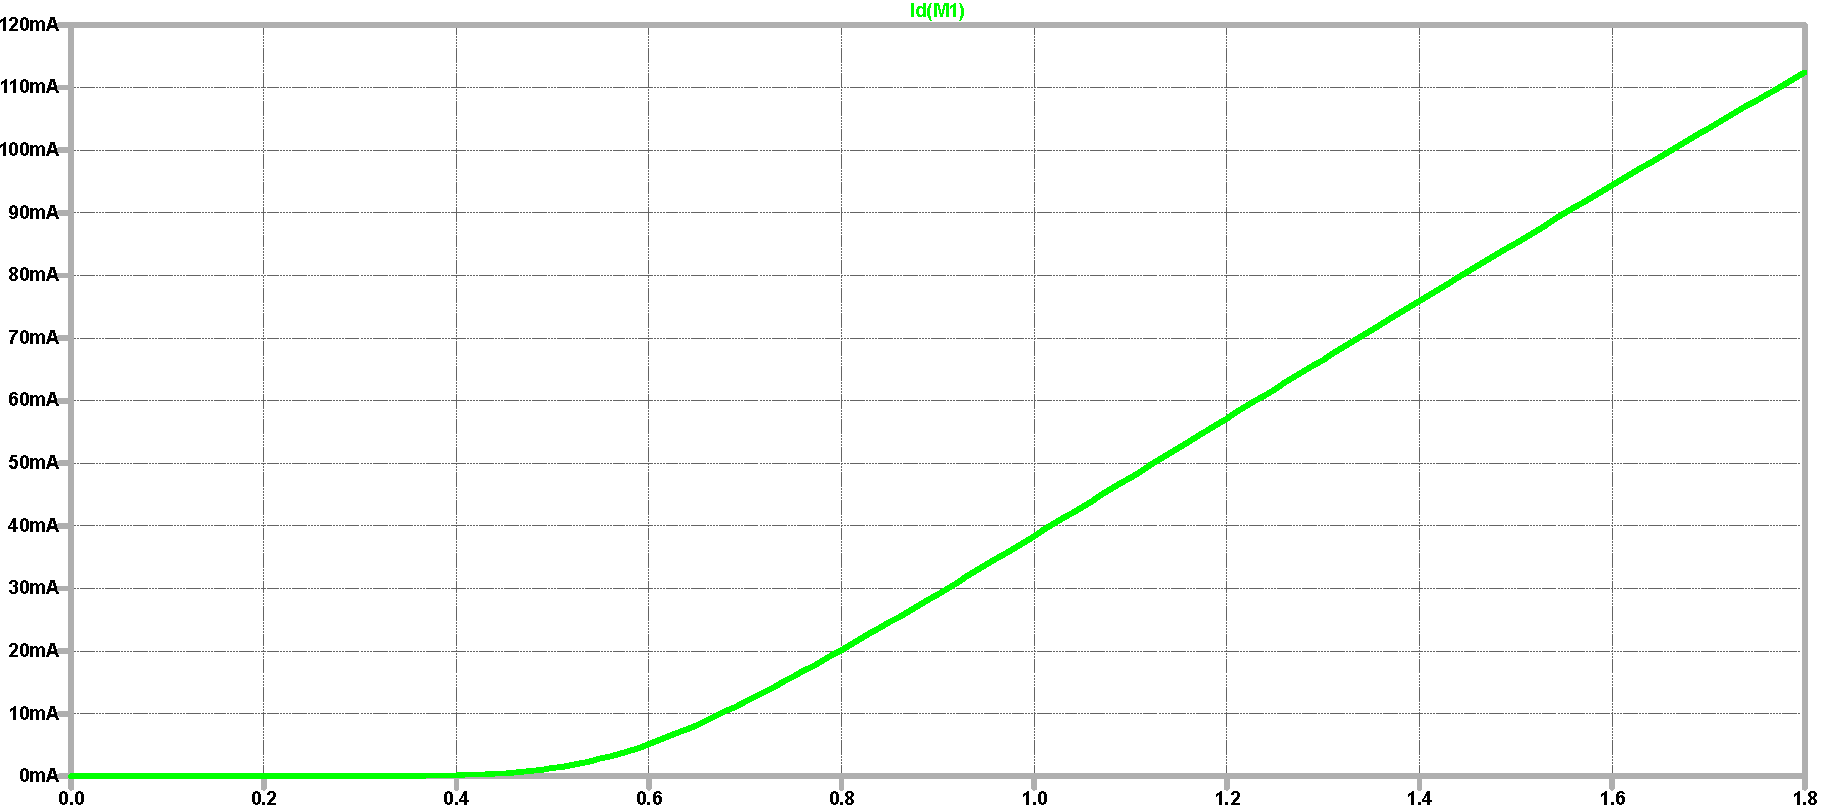
\includegraphics[width=.9\linewidth]{img/q1/id-vgs.pdf}
\caption{\label{fig:id-vgs-q1}\(I_{ds} - V_{gs}\) sweep}
\end{figure}

\item Impedance at low frequency:
\begin{enumerate}
\item Input, \(R_{in} = \infty \Omega{}\)

\item Output, \(R_{out} = r_{o} = \frac{1}{\lambda{} I_dmax} = 613 \Omega{}\)
\end{enumerate}

The simulated input and output impedance from LTspice are shown in \ref{fig:zin-zout-q1}.
It can be observed that \(Z_{in}\) tends to infinity at low frequencies, while Z\textsubscript{out} is
around \(603 \Omega{}\)

\begin{figure}[H]
\centering
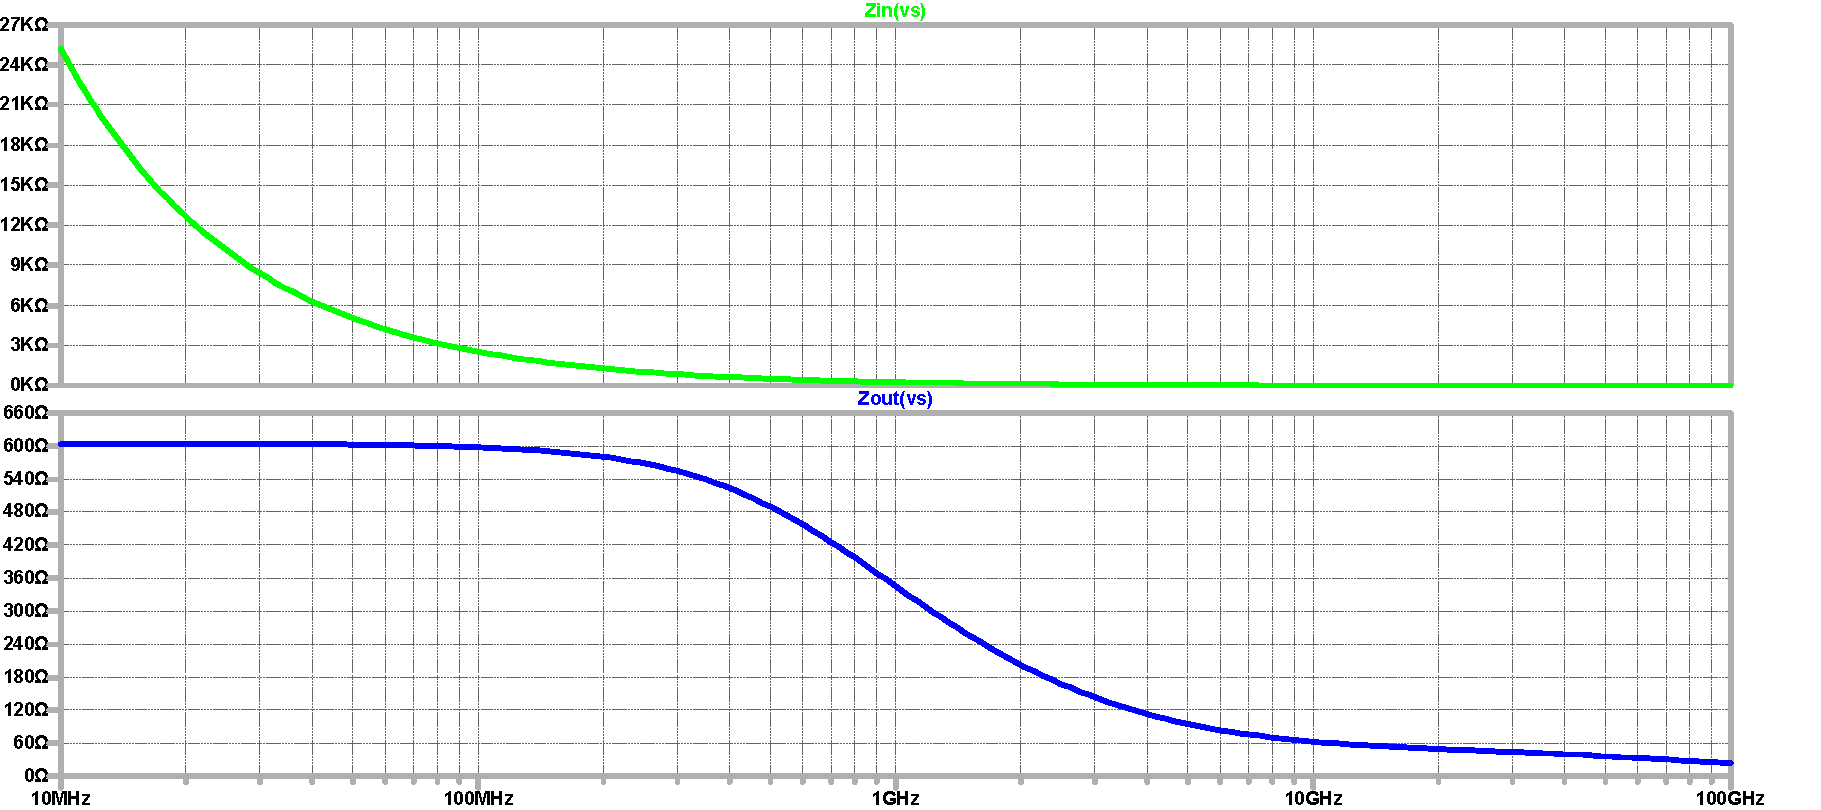
\includegraphics[width=.9\linewidth]{img/q1/zin-zout-d.pdf}
\caption{\label{fig:zin-zout-q1}\(Z_{in} and Z_{out} of amplifier\)}
\end{figure}

\item Capacitance of:
\begin{enumerate}[1.]
\item \(C_{gs}\)

\begin{equation*}
\begin{aligned}
C_{gs} &= \frac{2WLC_{OX}}{3} + WC_{OV} \\
&= \frac{2W_{g}LC_{OX}}{3} + W_{g}C_{OV} \\
&= 2.79 \times 10^{-13} F \\

\end{aligned}
\end{equation*}

\item \(C_{gd}\)

\begin{equation*}
\begin{aligned}
C_{gd} &= WC_{OV} \\
&= W_{g}C_{OV} \\
&= 7.32 \times 10^{-14} F \\
\end{aligned}
\end{equation*}
\end{enumerate}
\end{enumerate}

\subsection{Question 2}
\label{sec:org6626724}
\begin{enumerate}[A.]
\item Ohmic matching,
\begin{enumerate}[1]
\item Input
\begin{equation*}
\begin{aligned}
\frac{1}{R_{in,matched}} &= \frac{1}{R_{1}} + \frac{1}{R_{in}} \\
\frac{1}{50} &= \frac{1}{R_{1}} \\
R_{1} &= 50 \Omega \\
\end{aligned}
\end{equation*}

\item Output
\begin{equation*}
\begin{aligned}
\frac{1}{R_{out,matched}} &= \frac{1}{R_{2}} + \frac{1}{R_{out}} \\
\frac{1}{50} &= \frac{1}{R_{2}} + \frac{1}{603} \\
R_{2} &= 54.5 \Omega \\
\end{aligned}
\end{equation*}
\end{enumerate}

\item Expected gain
\begin{equation*}
\begin{aligned}
G_{m} = g_{m} &= 0.0774 S \\
R_{out} &= r_{o} // R_{2} // R_{L} \\
&= 25 \Omega \\
A_{V} &= -1.94 \\
\end{aligned}
\end{equation*}

\item Input capacitance
\begin{equation*}
\begin{aligned}
C_{in} &= C_{gs} + \frac{C_{ds}}{1-A_{V}} \\
&= 4.94 \times 10^{-13} F \\
\end{aligned}
\end{equation*}

\item Matching input inductance, \(L_{1}\).

Input impedance
\begin{equation*}
\begin{aligned}
%\frac{1}{Z_{in}} &= \frac{1}{R_{1} + sL_{1}} + sC_{in} \\
%Z_{in} &= \frac{R_{1} + sL_{1}}{1 + sR_{1}C_{in} - \omega^2L_{1}C_{in}} \\
%\\
L_{1} &\approx \frac{1}{\omega^2C_{IN}} \\
&= 1.69 \times 10^{-9} H \\
\end{aligned}
\end{equation*}
\end{enumerate}

\subsection{Question 3}
\label{sec:org7606ebc}
From previous section,
\begin{equation*}
\begin{aligned}
G_{m} = g_{m} &= 0.0774 S \\
R_{out} &= r_{o} // R_{2} // R_{L} \\
&= 25 \Omega \\
A_{V} &= -1.94 \\
\end{aligned}
\end{equation*}

Noise figure, \(F\),
\begin{equation*}
\begin{aligned}
F &= 1 + \frac{N_{a}}{N_{i}G} \\
\\
N_{i} &= \overline{v_{R_{s}}^{2}} \\
&= \frac{4kT}{R_{s}}(R_{s} // R_{in})^{2} \\
&= \frac{4kT}{R_{s}}(R_{s} // R_{1})^{2} \\
\\
N_{a} &= \overline{v_{R_{1}}^{2}} + \overline{v_{M}^{2}} + \overline{v_{R_{2}}^{2}} \\
&= \frac{4kTR_{1}(R_{s} // R_{in})^{2}}{R_{1}}A_{v}^{2} + (4kT\gamma{}g_{m} + \frac{4kT}{R_{2}})R_{out}^{2} \\
&= 4kT[\frac{(R_{S} // R_{1})^{2}}{R_{1}}A_{v}^{2} + (\gamma{}g_{m} + \frac{1}{R_{2}})R_{out}^{2}] \\
\\
F &= 1 + \frac{\frac{(R_{S} // R_{1})^{2}}{R_{1}}A_{v}^{2} + (\gamma{}g_{m} + \frac{1}{R_{2}})R_{out}^{2}}{\frac{[(R_{s} // R_{1})A_{v}]^{2}}{R_{s}}} \\
&= 2.93 \\
&= 4.6 dB \\

\end{aligned}
\end{equation*}

\subsection{Question 4}
\label{sec:orge3a9c9b}
\begin{enumerate}[A.]
\item Ohmic matching. If the circuit is correctly matched the real part of the input impedance,
\(Re\{Z_{in}(f = 5.5GHz)\} = 50 \Omega\),
the real part of the output impedance, \(Re\{Z_{out}(f = 5.5GHz)\} = 50 \Omega\).
The simulated \(Z_{in}\) and \(Z_{out}\) are shown in Figure \ref{fig:zin-zout-q4},
the matched impedance values are shown in \ref{tab:zin-zout-q4}.

Since the resistance will also affect the resonanance frequency of an RLC circuit,
the fine tuned values used are shown in Table \ref{tab:param-q4}.

\item Reactance matching. If the circuit is correctly matched the imaginary part of the input impedance,
\(Im\{Z_{in}(f = 5.5GHz)\} = 0 \Omega\),
the imaginary part of the output impedance, \(Im\{Z_{out}(f = 5.5GHz)\} = 0 \Omega\).
The simulated \(Z_{in}\) and \(Z_{out}\) are shown in Figure \ref{fig:zin-zout-q4},
the matched impedance values are shown in \ref{tab:zin-zout-q4}.

Since the resistance will also affect the resonanance frequency of an RLC circuit,
the fine tuned values used are shown in Table \ref{tab:param-q4}.

\begin{table}[htbp]
\caption{\label{tab:zin-zout-q4}Matched impedance at \(f = 5.5GHz\)}
\centering
\begin{tabular}{ll}
\hline
Impedance & Value\\
\hline
\(Z_{in}\) & \(49.97 - 0.13i \Omega\)\\
\(Z_{out}\) & \(49.69 - 0.15i \Omega\)\\
\hline
\end{tabular}
\end{table}

\begin{table}[htbp]
\caption{\label{tab:param-q4}Impedance matching parameters}
\centering
\begin{tabular}{ll}
\hline
Parameter & Value\\
\hline
\(R_{1}\) & \(49 \Omega\)\\
\(R_{2}\) & \(53 \Omega\)\\
\(L_{1}\) & \(1.65 nH\)\\
\(L_{2}\) & \(3.99 nH\)\\
\hline
\end{tabular}
\end{table}

\begin{figure}[H]
\centering
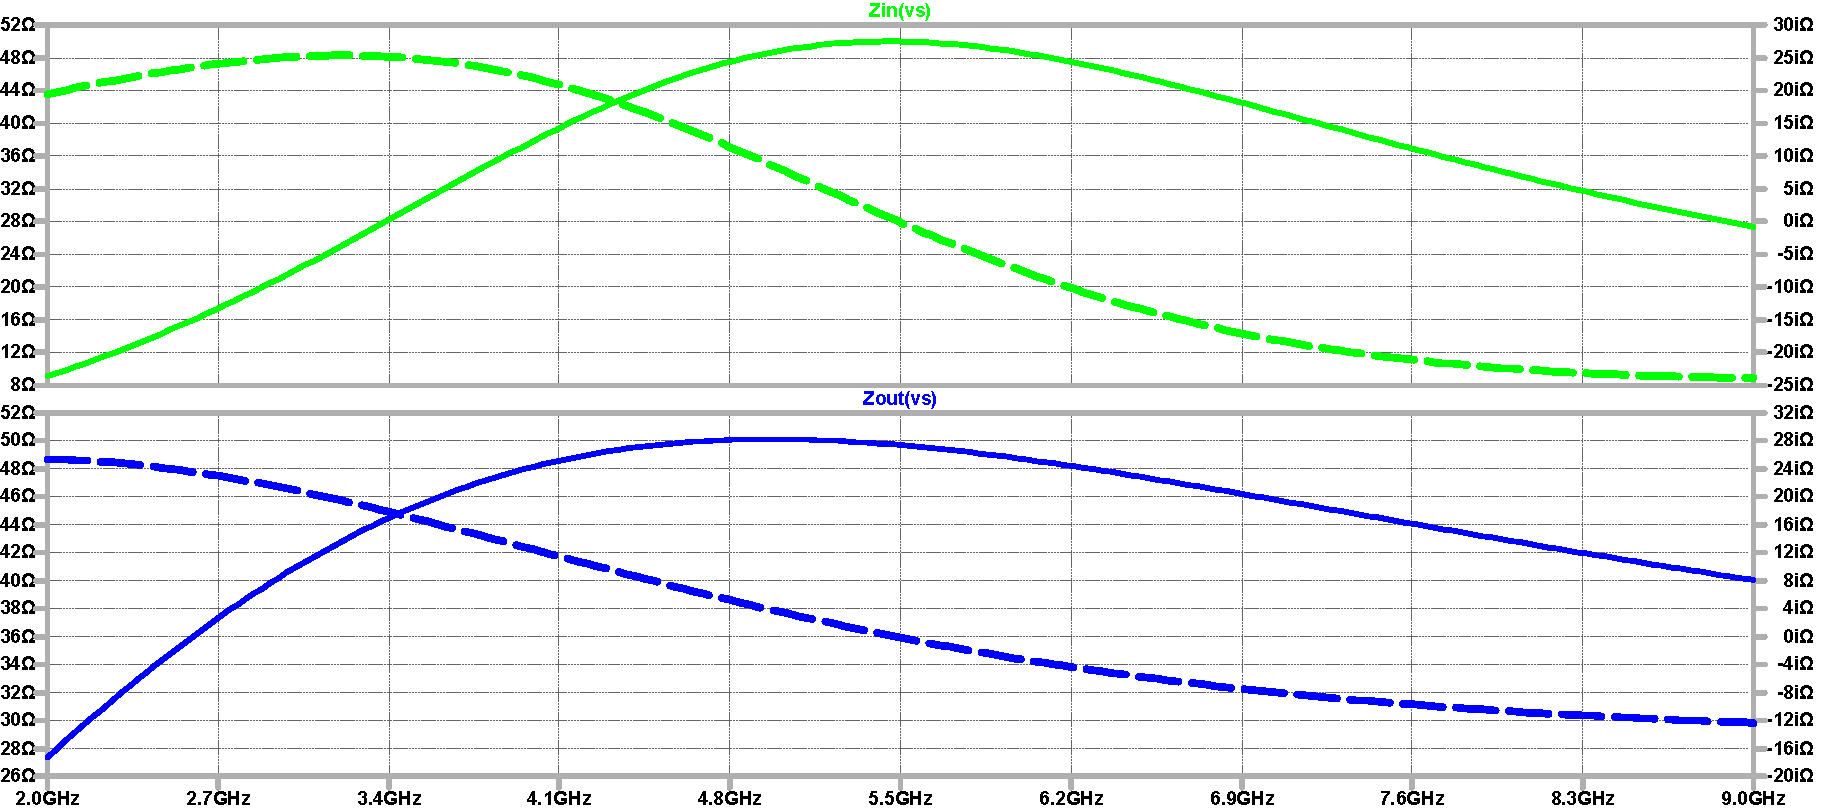
\includegraphics[width=.9\linewidth]{img/q4/zin-zout.pdf}
\caption{\label{fig:zin-zout-q4}\(Z_{in}\) and \(Z_{out}\)}
\end{figure}

\item S-parameters,
\begin{enumerate}[1)]
\item No matching
\begin{figure}[H]
\centering
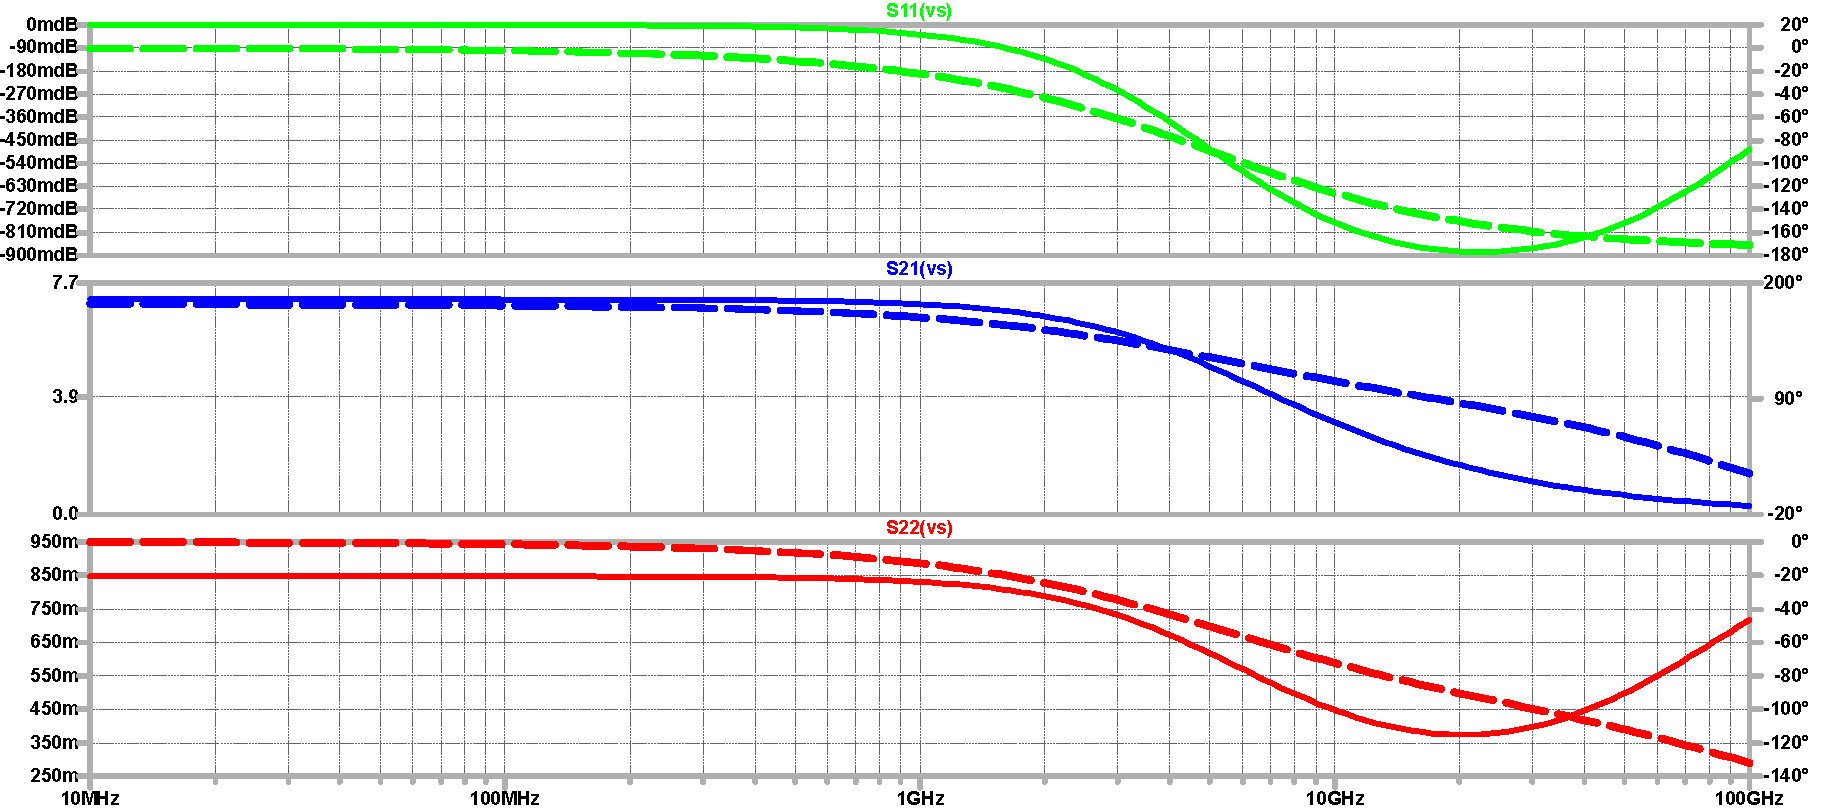
\includegraphics[width=.9\linewidth]{img/q4/s-unmatched.pdf}
\caption{\label{fig:s-unmatched-q4}S-parameters without matching}
\end{figure}

\item Ohmic matching
\begin{figure}[H]
\centering
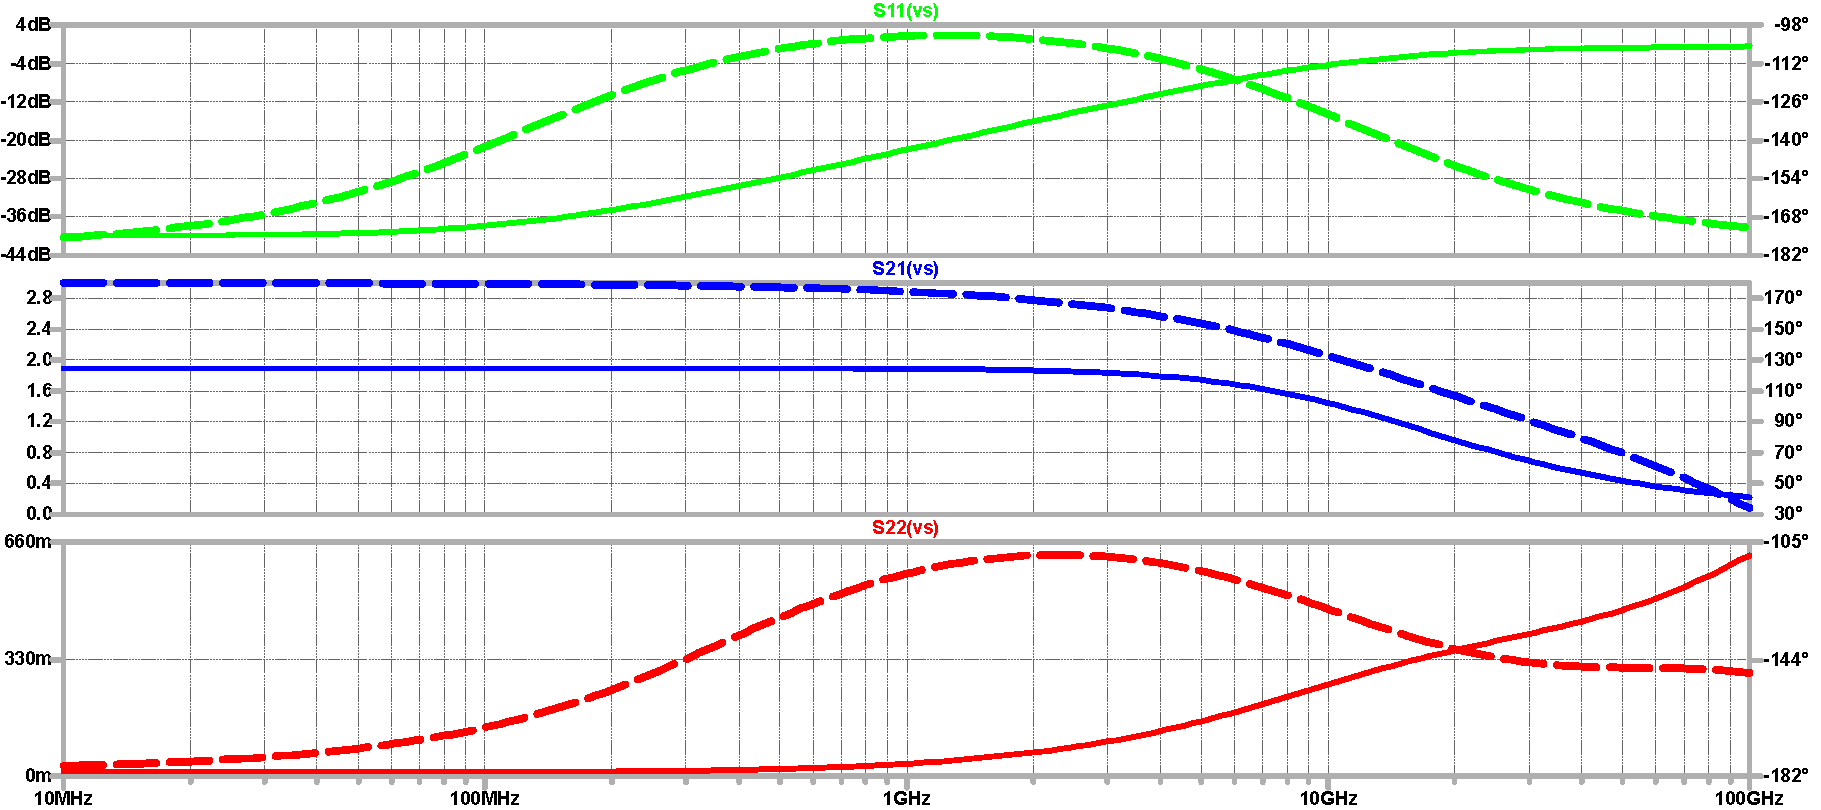
\includegraphics[width=.9\linewidth]{img/q4/s-r-matched.pdf}
\caption{\label{fig:s-r-match-q4}S-parameters with ohmic matching}
\end{figure}

\item Ohmic and conjugate matching
\begin{figure}[H]
\centering
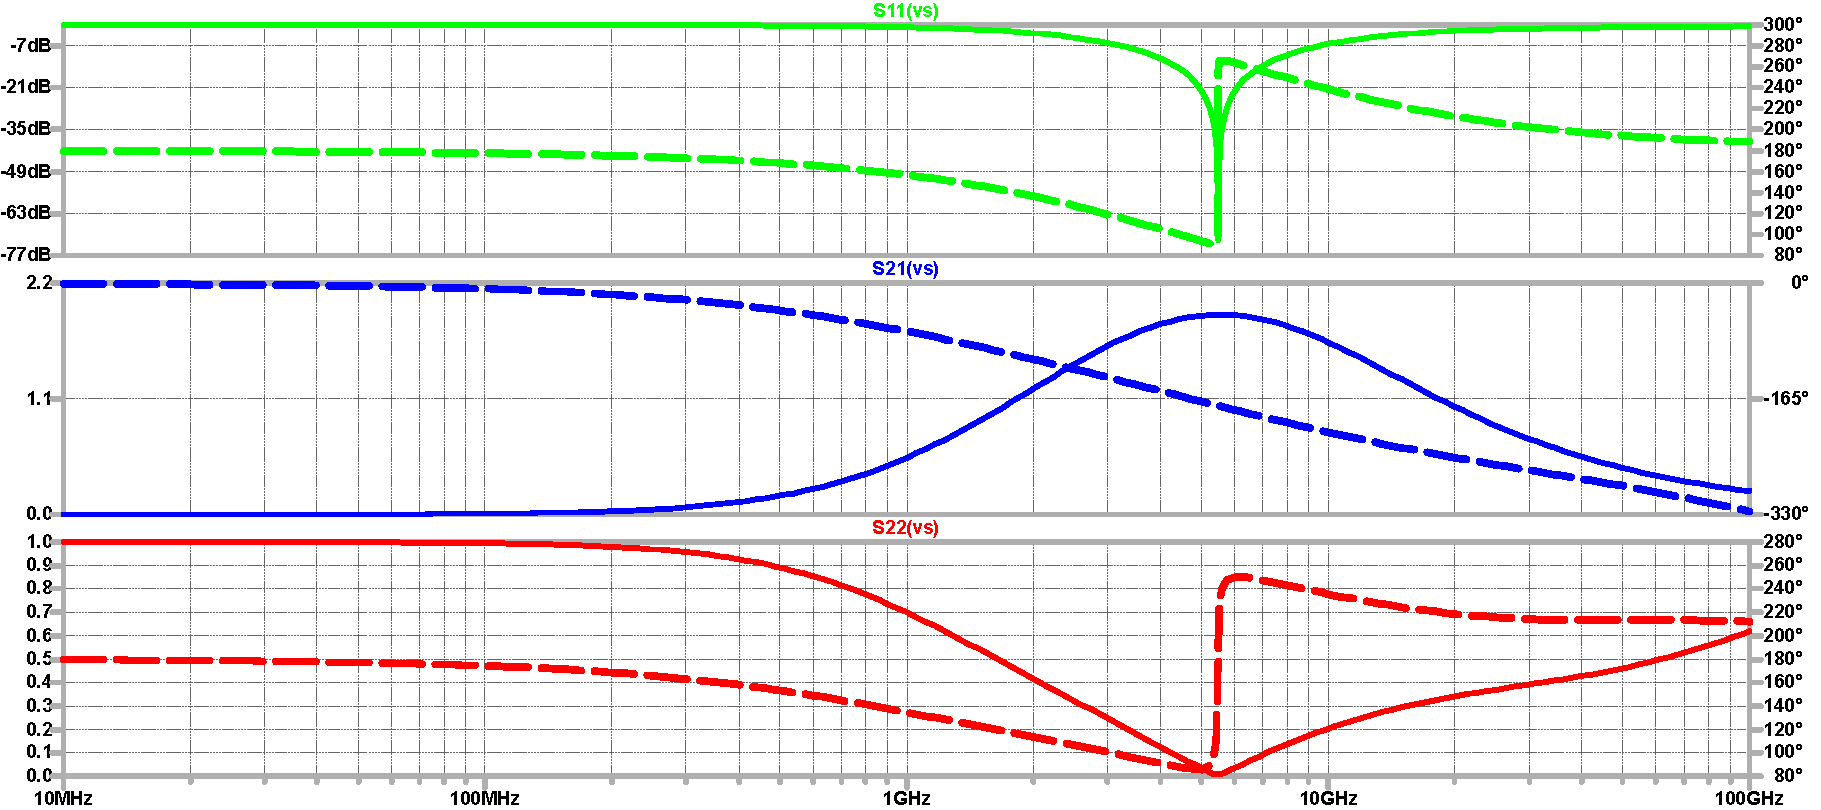
\includegraphics[width=.9\linewidth]{img/q4/s-matched.pdf}
\caption{\label{fig:s-matched-q4}S-parameters with ohmic and conjugate matching}
\end{figure}
\end{enumerate}

\item Noise Factor,
\begin{enumerate}[1)]
\item No matching
\begin{figure}[H]
\centering
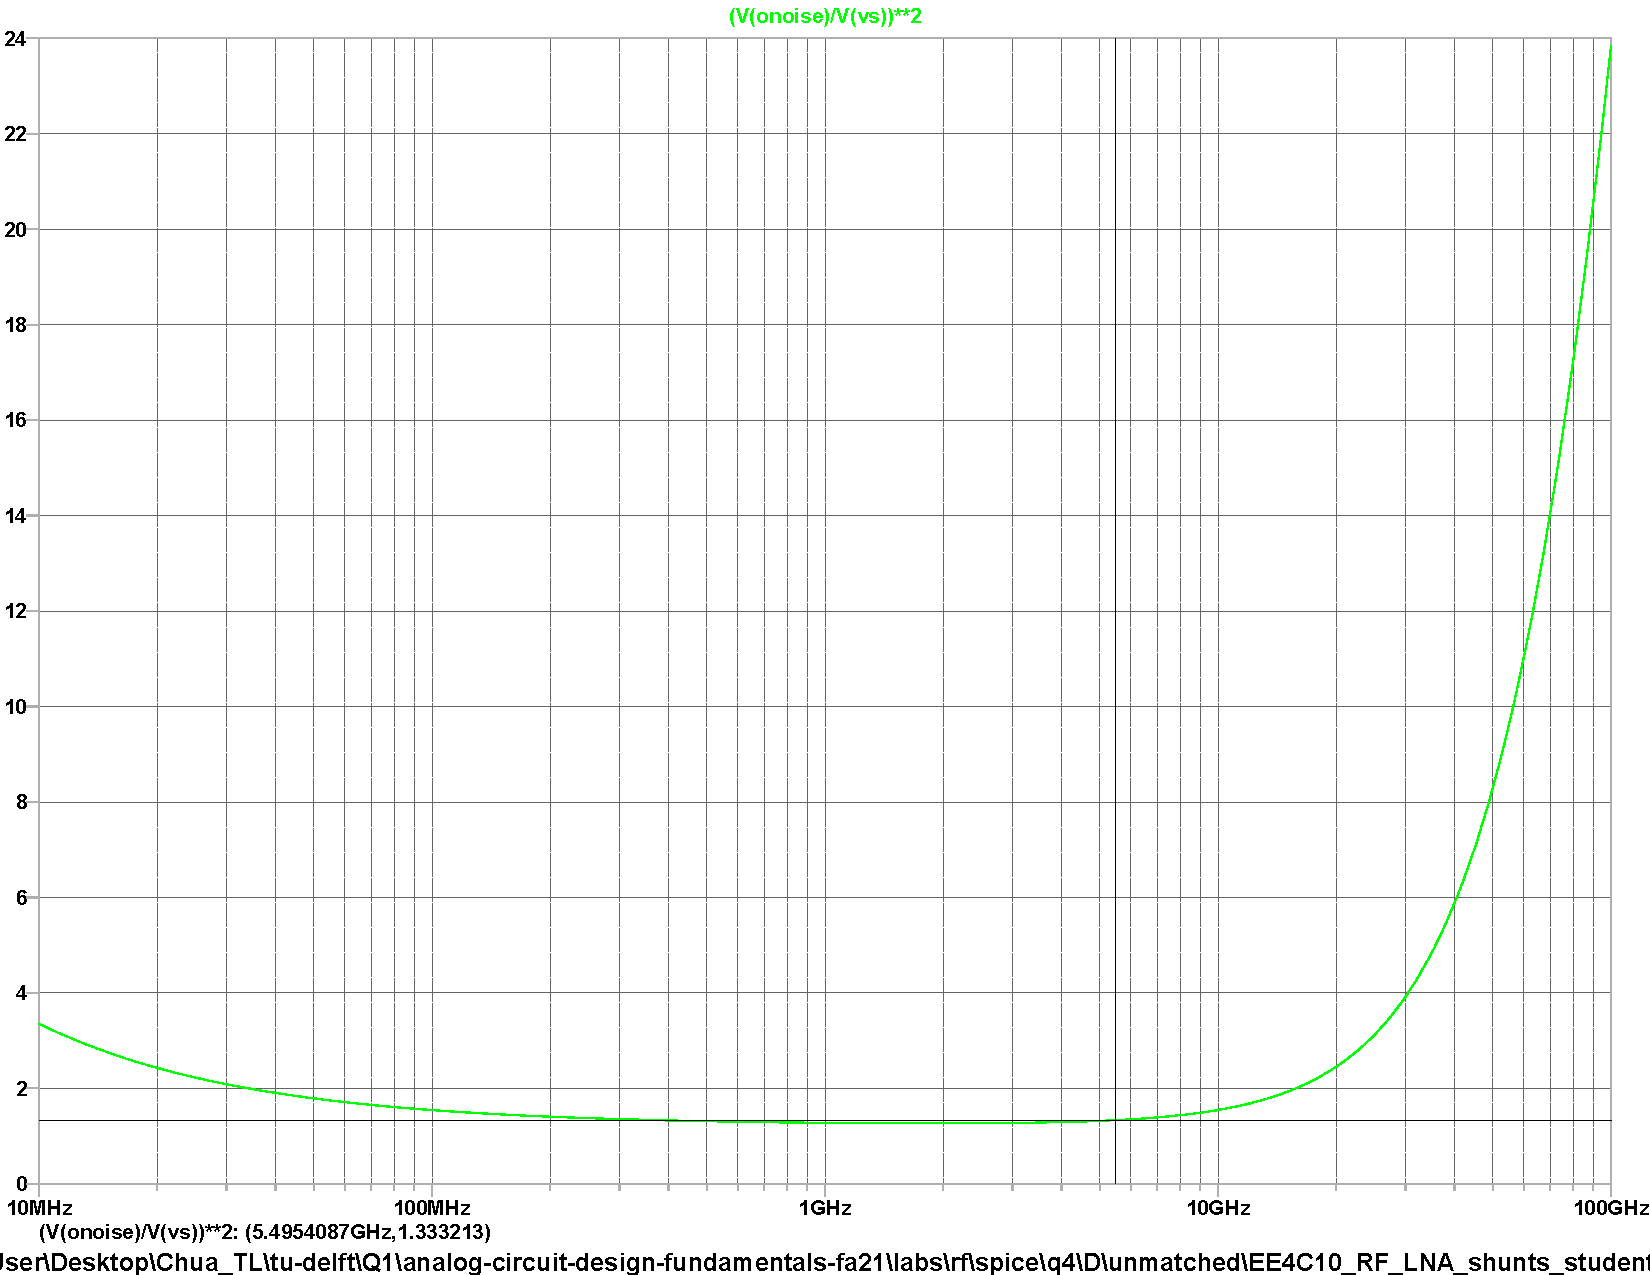
\includegraphics[height=300px]{img/q4/noise-unmatched-2.pdf}
\caption{\label{fig:noise-unmatched-q4}Noise Factor without matching}
\end{figure}

\item Ohmic matching
\begin{figure}[H]
\centering
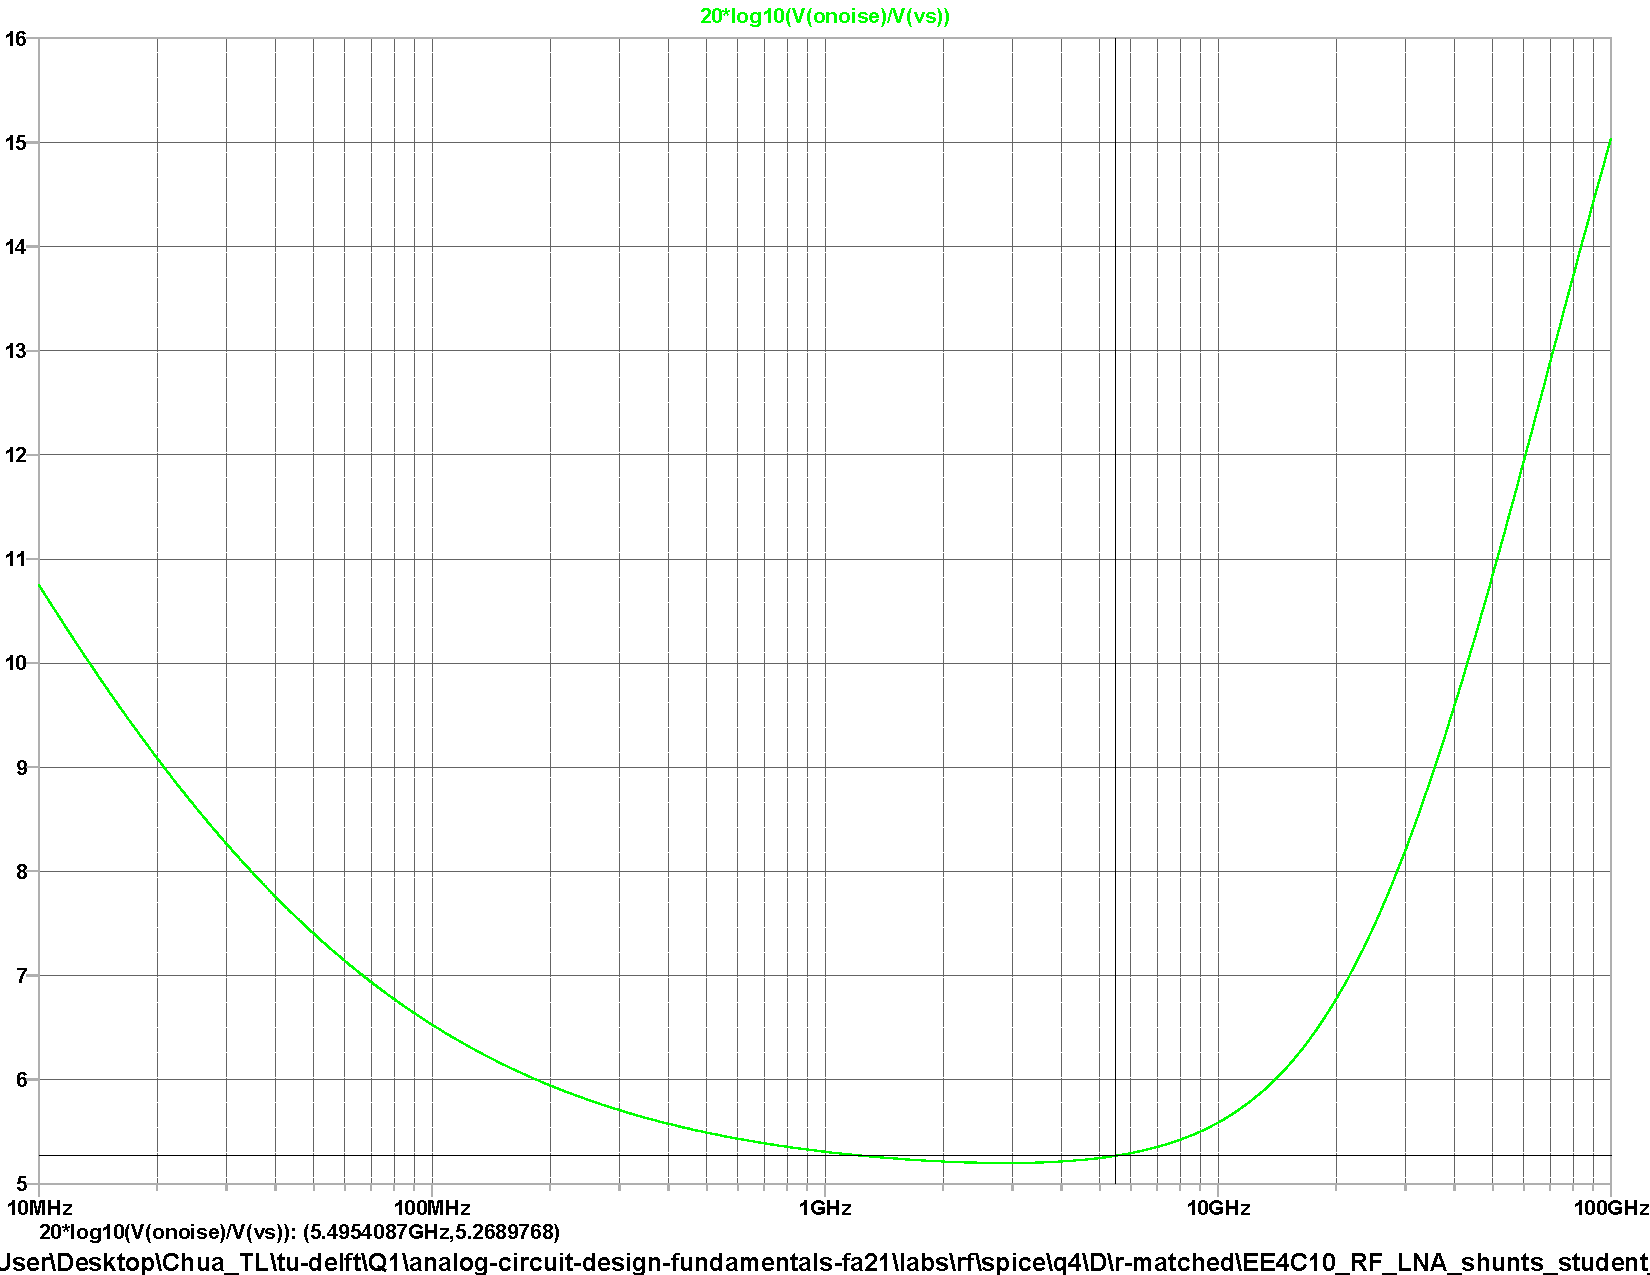
\includegraphics[height=300px]{img/q4/noise-r-matched-2.pdf}
\caption{\label{fig:noise-r-match-q4}Noise Factor with ohmic matching}
\end{figure}

\item Ohmic and conjugate matching
\begin{figure}[H]
\centering
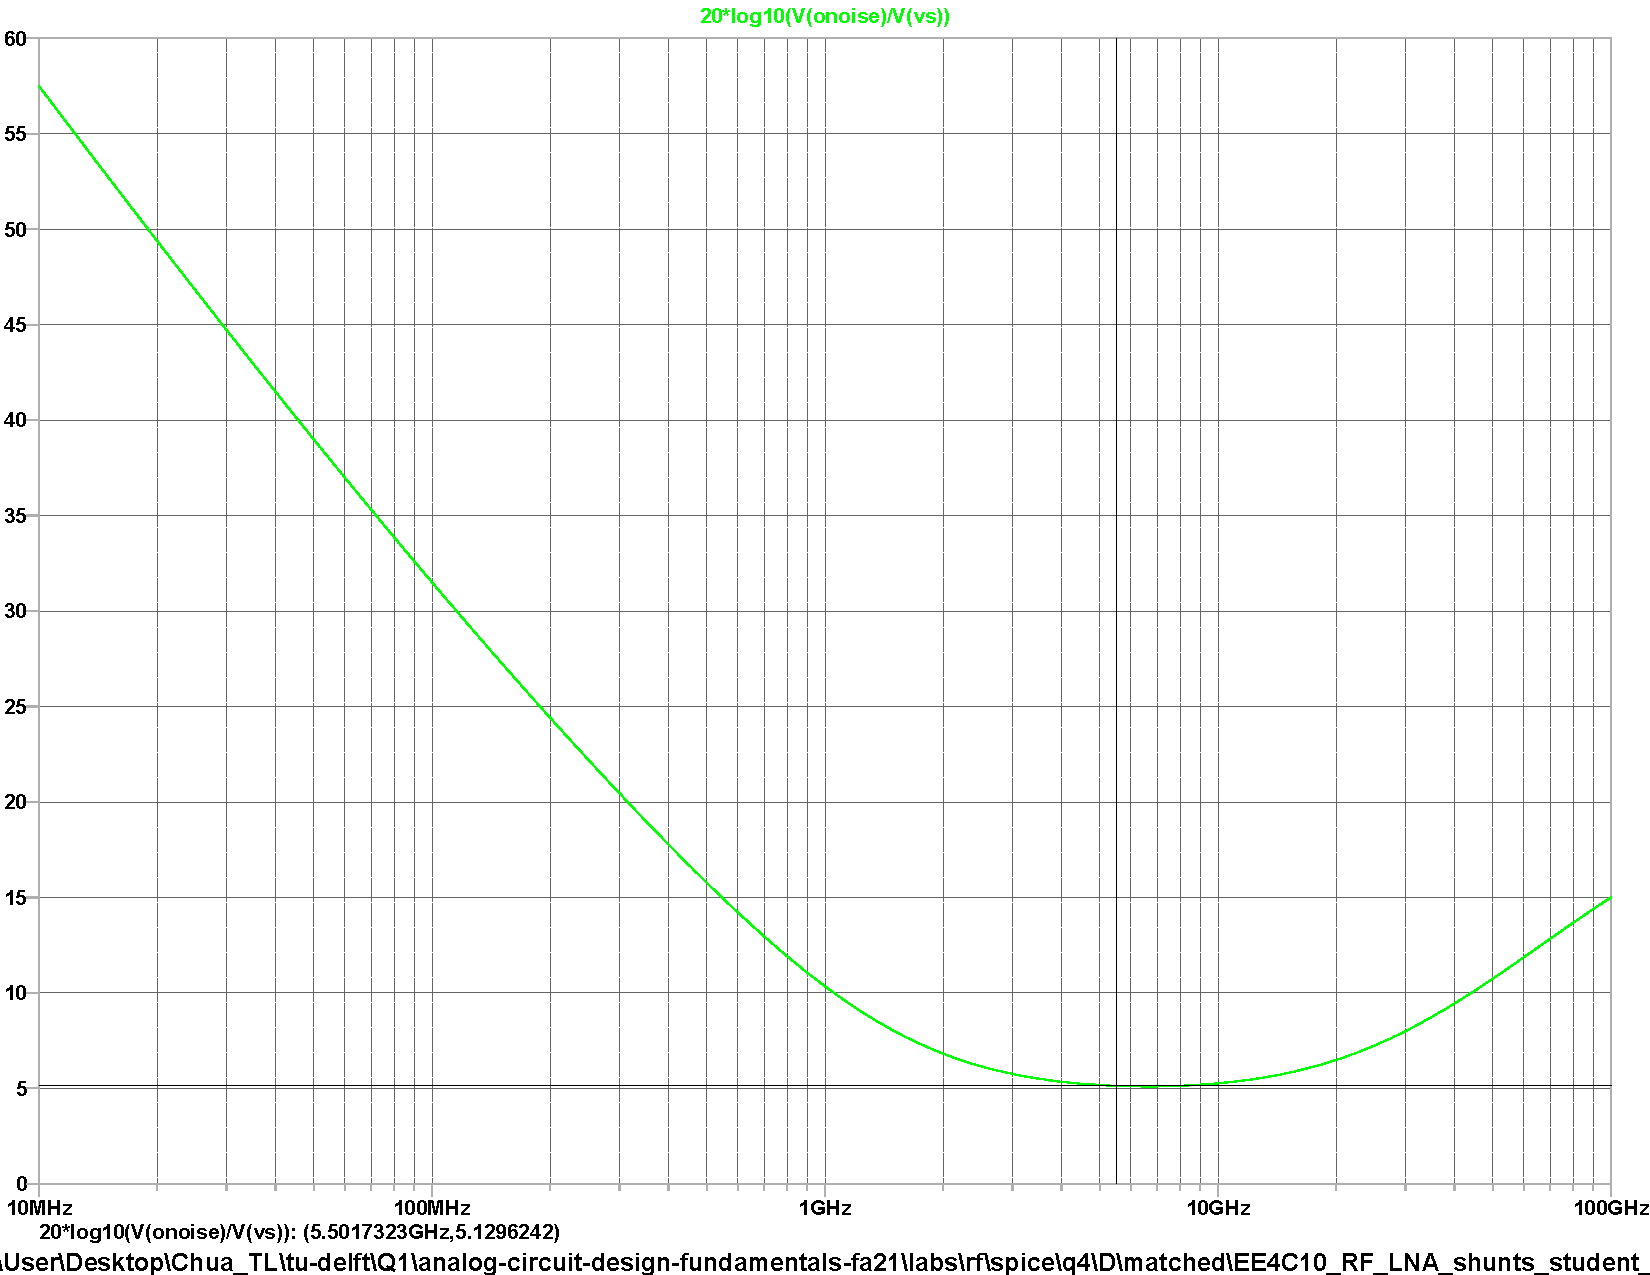
\includegraphics[height=300px]{img/q4/noise-matched-2.pdf}
\caption{\label{fig:noise-matched-q4}Noise Factor with ohmic and conjugate matching}
\end{figure}
\end{enumerate}

\item LNA performance using simplistic ``design method''.
\begin{enumerate}[1)]
\item Advantages

\begin{itemize}
\item Low refection coefficient, \(S_{11} = -71 dB\).
\item Simple matching procedure due to uncorrelated input and output.
\end{itemize}

\item Disadvantages.

\begin{itemize}
\item Low gain, \(S_{21} = 1.9 dB\).

\item High noise figure of \(F \approx 5dB\).

\item The bandwith of the amplifier is small.
\end{itemize}
\end{enumerate}
\end{enumerate}


\section{Part 2}
\label{sec:orgb499591}
\subsection{Question 5}
\label{sec:org9338ea6}
\begin{enumerate}[A.]
\item From Question 1, the gate width, \(W_{g}\), and gate bias voltage, \(V_{gs}\),
\begin{equation*}
\begin{aligned}
W_{g} &= 200 \mu{}m \\
V_{gs} &= 0.7 V \\
\end{aligned}
\end{equation*}

Input impedance of LNA,
\begin{equation*}
\begin{aligned}
R_{in} &= \frac{V_{X}}{I_{X}} \\
\\
g_{m}V_{x} + \frac{V_{x} - I_{x}(R_{f}r_{o})}{r_{o}R_{L}} &= I_{x} \\
V_{x}(g_{m} + \frac{r_{o} + R_{L}}{r_{o}R_{L}}) &= I_{X}(1 + \frac{R_{f}(r_{o} + R_{L})}{r_{o}R_{L}}) \\
R_{f} &= \frac{R_{in}(r_{o} + R_{L} + g_{m}r_{o}R_{m}) - r_{o}R_{L}}{r_{o} + R_{L}} \\
&= 182 \Omega \\
\end{aligned}
\end{equation*}

\item The input impedance is matched using the reseistance of the single loop feedback,
however, the output impedance is still unmatched. Since the task is to only match the input impedance,
a single-loop feedback is sufficient.

\item Methods for improving the performance of the single loop feedback:
\begin{itemize}
\item Using a cascode-stage. The input and output impedancences will be isolated,
which will aid in the input and output impedance matching. However, the bias volatage has to be
increased to maintain the current budget.

\item Adding an extra stage for increasing the overall gain of the amplifier, this will increase the power
consumption.

\item From the slides, the 2 methods above can be combined with adding ``phantom zeros'' to increase or provide sufficient
the gain bandwidth, which in the current design lacks.
\end{itemize}
\end{enumerate}


\subsection{Question 6}
\label{sec:org7f8d6c7}
\begin{enumerate}[A.]
\item Input and output impedance with \(R_{f} = 182 \Omega\).

\begin{figure}[H]
\centering
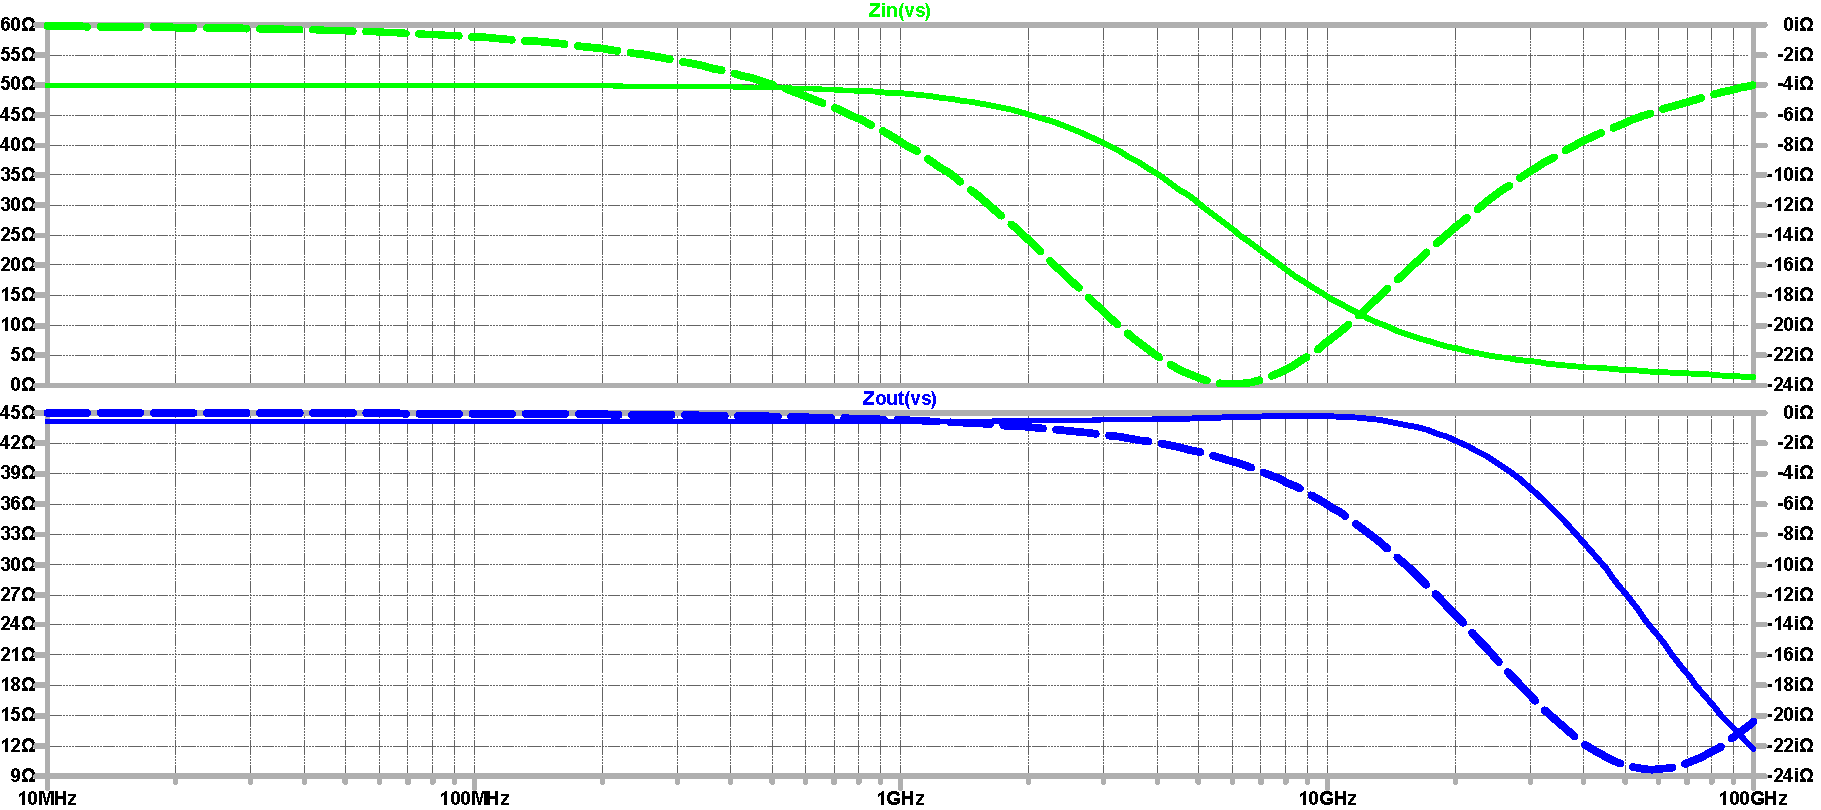
\includegraphics[width=.9\linewidth]{img/q6/zin-zout-r-matched.pdf}
\caption{\label{fig:zin-zout-r-matched-q6}Input and output impedance with resistive feedback, \(R_{f} = 182 \Omega\).}
\end{figure}

\item S-Parameters with \(R_{f} = 182 \Omega\).

\begin{figure}[H]
\centering
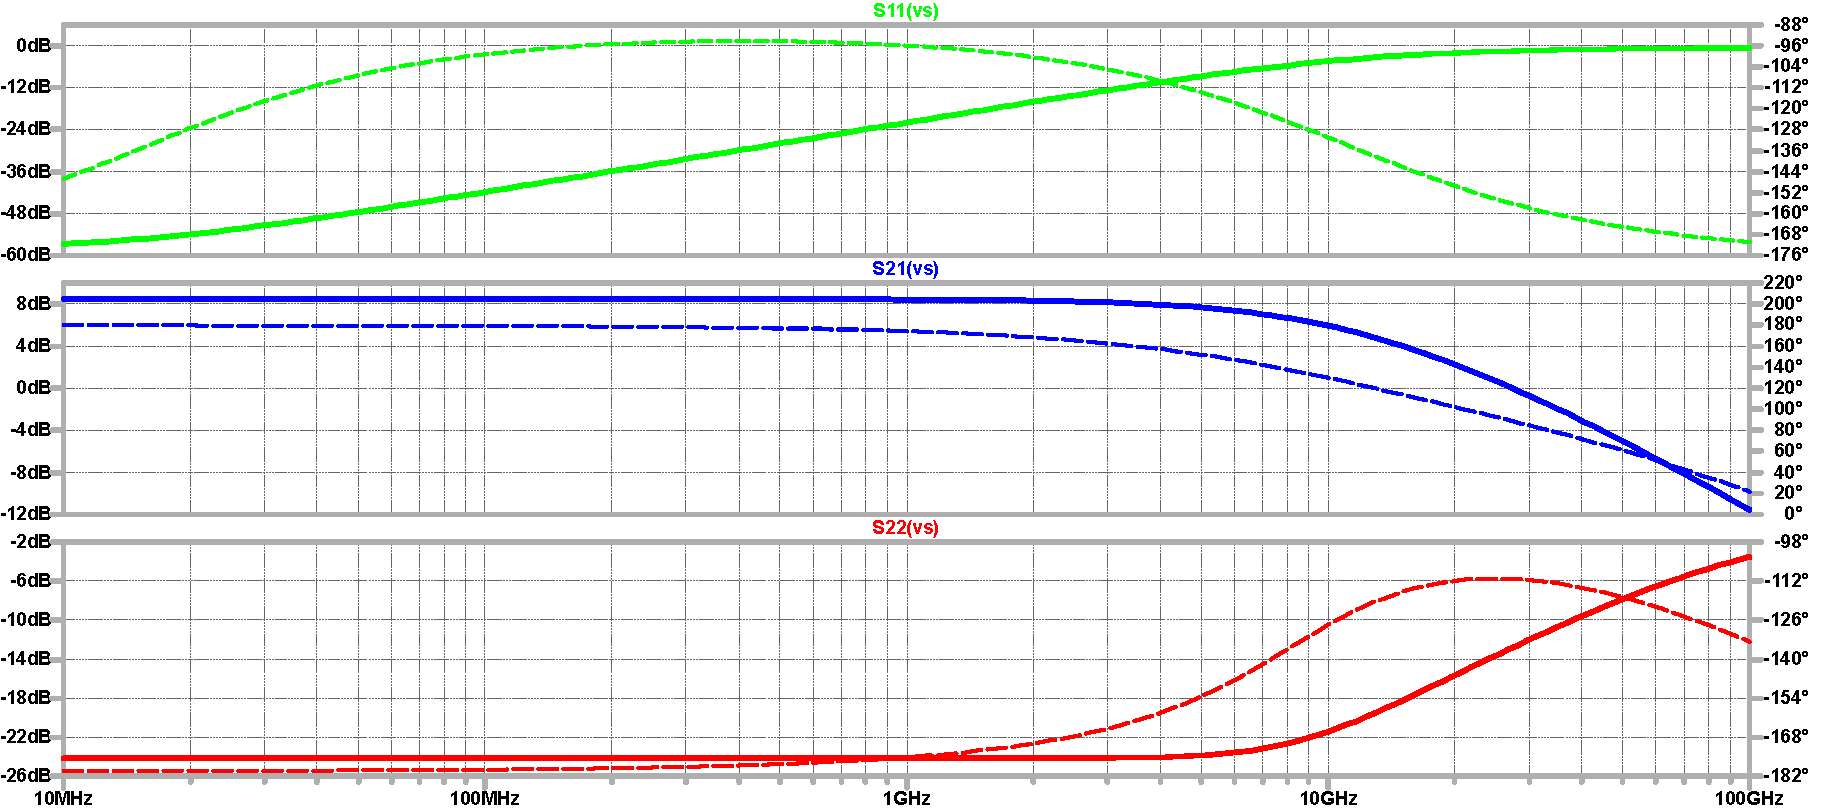
\includegraphics[width=.9\linewidth]{img/q6/s-r-matched.pdf}
\caption{\label{fig:s-r-matched-q6}S-parameters with resistive feedback, \(R_{f} = 182 \Omega\).}
\end{figure}

\item Noise figure with \(R_{f} = 182 \Omega\).

\begin{figure}[H]
\centering
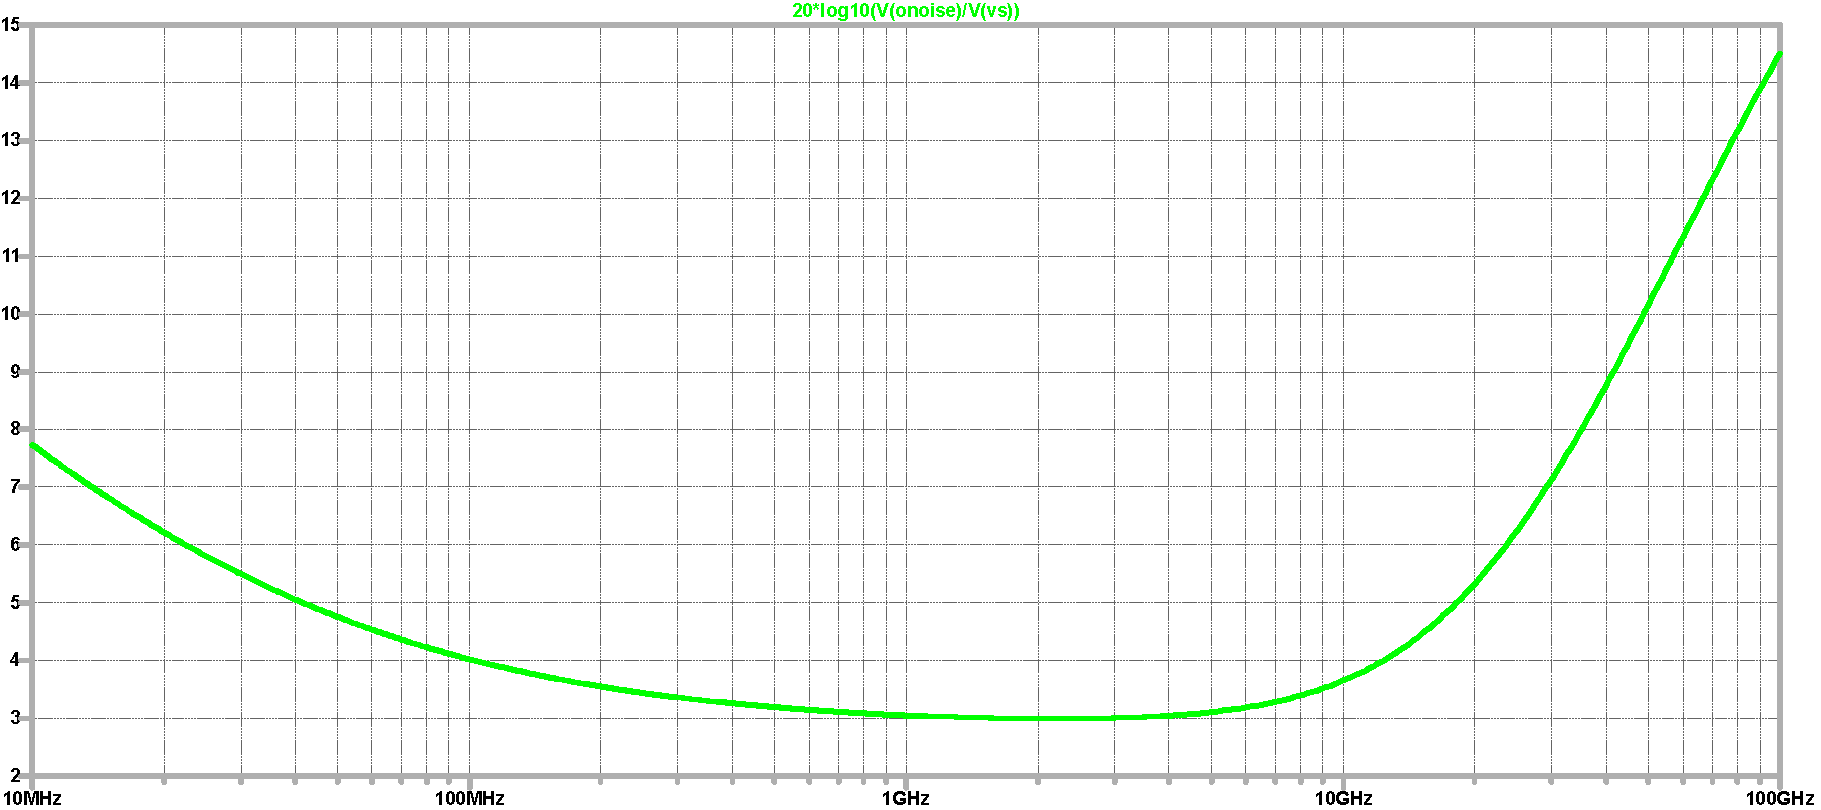
\includegraphics[width=.9\linewidth]{img/q6/noise-r-matched.pdf}
\caption{\label{fig:noise-r-matched-q6}Noise figure with resistive feedback, \(R_{f} = 182 \Omega\).}
\end{figure}

\item 2 methods were attempted for designing the LNA:
\begin{enumerate}
\item Matching \(Z_{in} \approx 50 \Omega\) and \(Z_{out} \approx 50 \Omega\) at 5.5GHz.
After some fine tuning, the matching element values are shown in Table \ref{tab:param-q6d1}.
The specifications of the resulting LNA are shown in Table \ref{tab:specs-q6d1}, with the simulated results in
Figure \ref{fig:zin-zout-z-matched-q6}, \ref{fig:s-param-z-matched-q6}, and \ref{fig:noise-z-matched-q6}.
\begin{table}[htbp]
\caption{\label{tab:param-q6d1}Impedance matching parameters for \(Z_{in} \approx 50 \Omega\) and \(Z_{out} \approx 50 \Omega\)}
\centering
\begin{tabular}{ll}
\hline
Parameter & Value\\
\hline
\(R_{f}\) & \(154 \Omega\)\\
\(L_{in}\) & \(1.2 nH\)\\
\(L_{out}\) & \(2 nH\)\\
\hline
\end{tabular}
\end{table}

\begin{table}[htbp]
\caption{\label{tab:specs-q6d1}LNA Specifications for matching parameters for \(Z_{in} \approx 50 \Omega\) and \(Z_{out} \approx 50 \Omega\)}
\centering
\begin{tabular}{ll}
\hline
Parameter & Value\\
\hline
\(Z_{in}\) & \(54.0 + 1.2i \Omega\)\\
\(Z_{out}\) & \(47.9 + 0.9i \Omega\)\\
\(S_{11}\) & \(-27.7 dB\)\\
Gain, \(S_{21}\) & \(7.64 dB\)\\
\(S_{22}\) & \(-32.7 dB\)\\
Bandwidth, \(BW\) & \(> 1 GHz\)\\
Noise Figure, \(F\) & \(3.4 dB\)\\
\hline
\end{tabular}
\end{table}

\begin{figure}[H]
\centering
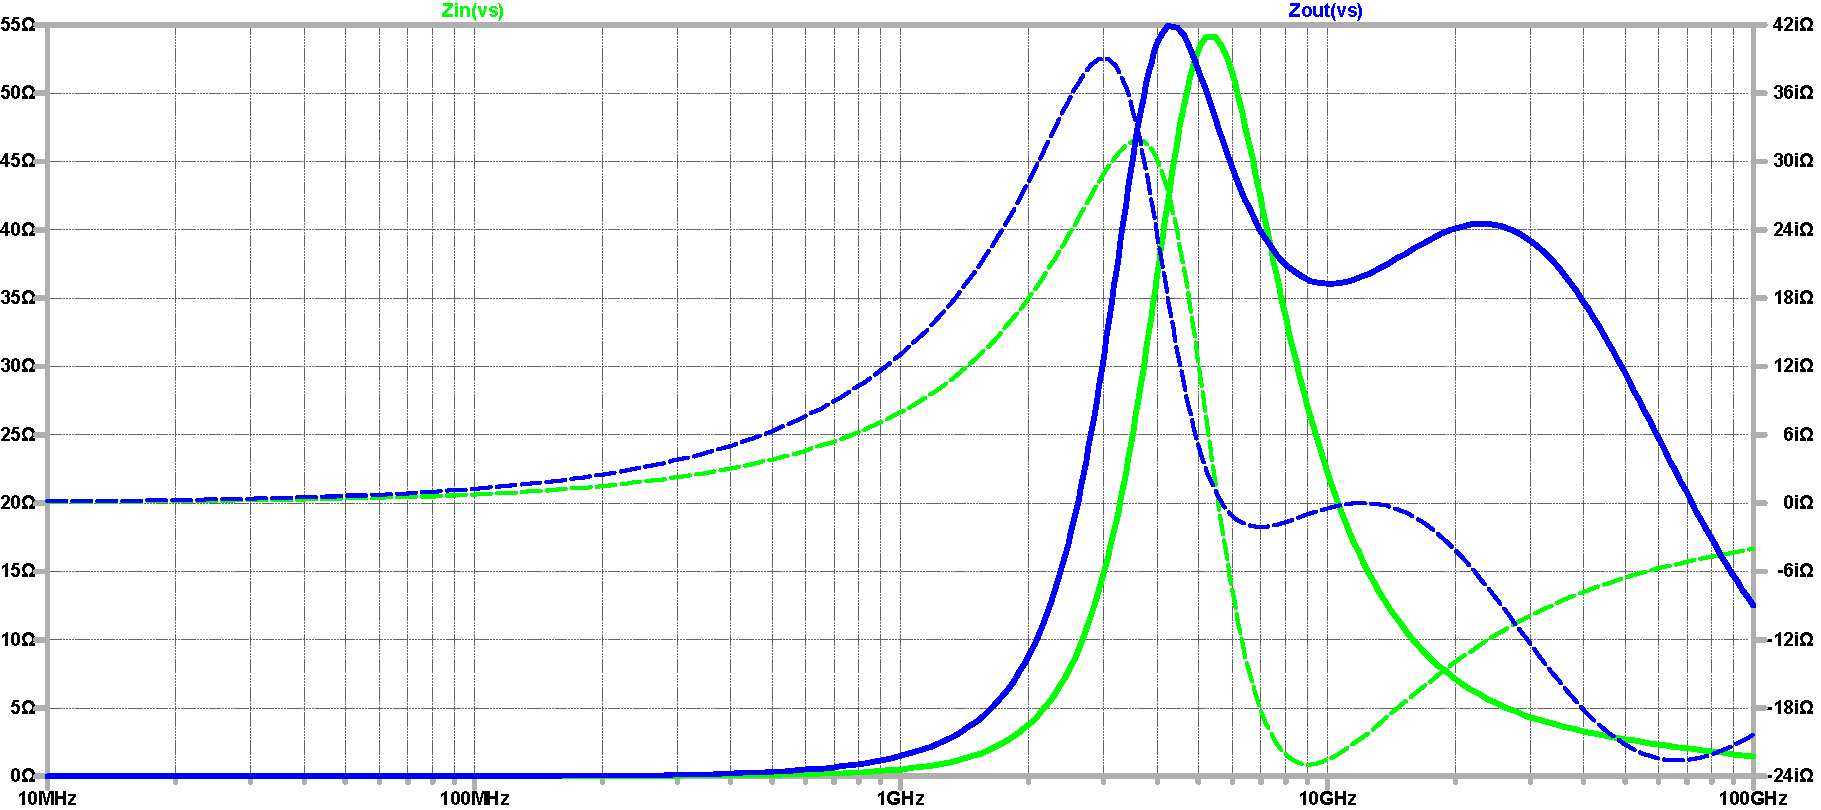
\includegraphics[width=.9\linewidth]{img/q6/zin-zout-z-matched.pdf}
\caption{\label{fig:zin-zout-z-matched-q6}Input and output impedance with \(Z_{in} \approx 50 \Omega\) and \(Z_{out} \approx 50 \Omega\)}
\end{figure}

\begin{figure}[H]
\centering
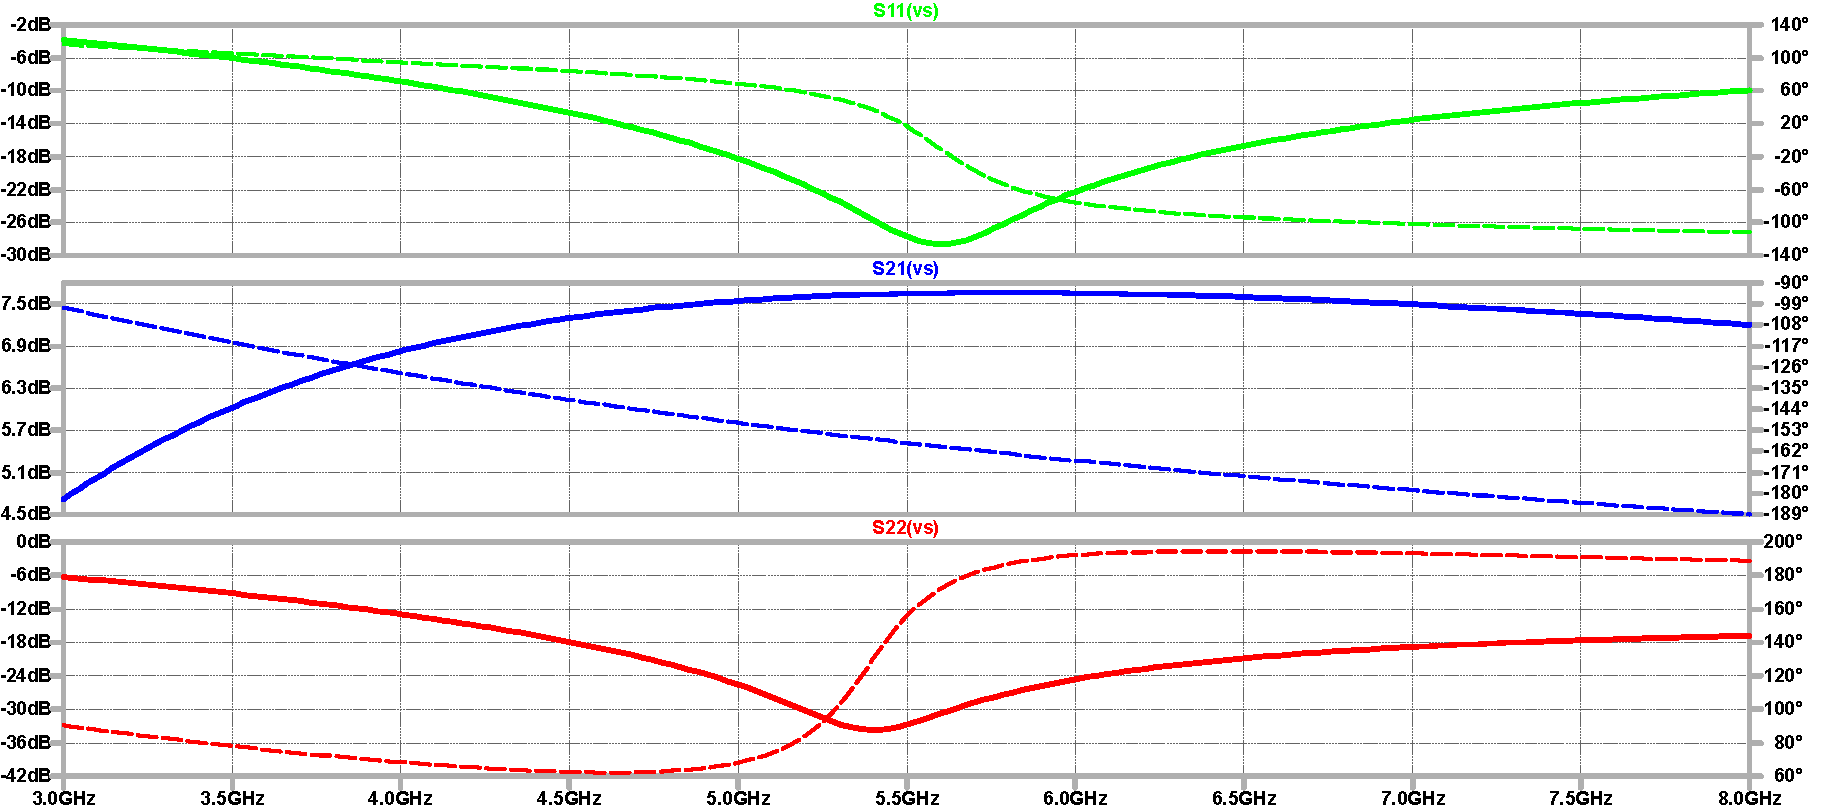
\includegraphics[width=.9\linewidth]{img/q6/s-z-matched.pdf}
\caption{\label{fig:s-param-z-matched-q6}S-parameters with \(Z_{in} \approx 50 \Omega\) and \(Z_{out} \approx 50 \Omega\)}
\end{figure}

\begin{figure}[H]
\centering
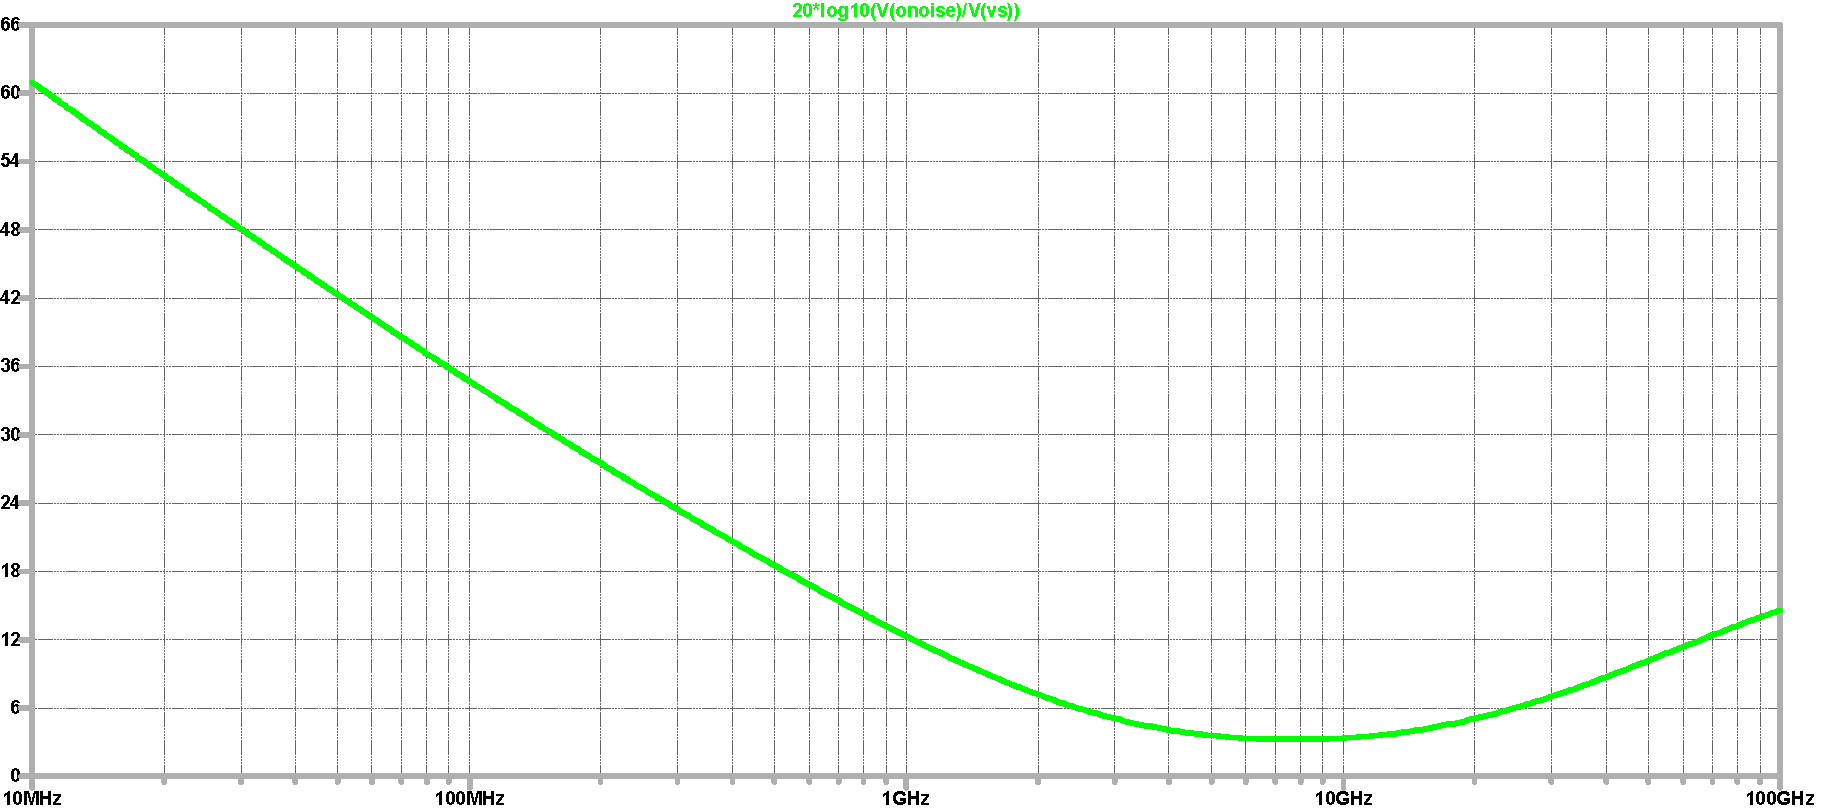
\includegraphics[width=.9\linewidth]{img/q6/noise-z-matched.pdf}
\caption{\label{fig:noise-z-matched-q6}Noise figure with \(Z_{in} \approx 50 \Omega\) and \(Z_{out} \approx 50 \Omega\)}
\end{figure}

\item Matching the minimum of S11 and S22 to be at 5.5GHz.
After some fine tuning, the matching element values are shown in Table \ref{tab:param-q6d2}.
The specifications of the resulting LNA are shown in Table \ref{tab:specs-q6d1}, with the simulated results in
Figure \ref{fig:zin-zout-s-matched-q6}, \ref{fig:s-param-s-matched-q6}, and \ref{fig:noise-s-matched-q6}.
\begin{table}[htbp]
\caption{\label{tab:param-q6d2}Impedance matching parameters for minimum S\textsubscript{11} and S\textsubscript{22}.}
\centering
\begin{tabular}{ll}
\hline
Parameter & Value\\
\hline
\(R_{f}\) & \(182 \Omega\)\\
\(L_{in}\) & \(1.3 nH\)\\
\(L_{out}\) & \(2.5 nH\)\\
\hline
\end{tabular}
\end{table}

\begin{table}[htbp]
\caption{\label{tab:specs-q6d1}LNA Specifications for matching parameters with minimum S\textsubscript{11} and S\textsubscript{22}.}
\centering
\begin{tabular}{ll}
\hline
Parameter & Value\\
\hline
\(Z_{in}\) & \(58.8 - 2.5i \Omega\)\\
\(Z_{out}\) & \(52.3 - 5.2i \Omega\)\\
\(S_{11}\) & \(-21.6 dB\)\\
Gain, \(S_{21}\) & \(8.7 dB\)\\
\(S_{22}\) & \(-25.1 dB\)\\
Bandwidth, \(BW\) & \(> 1 GHz\)\\
Noise Figure, \(F\) & \(3.0 dB\)\\
\hline
\end{tabular}
\end{table}

\begin{figure}[H]
\centering
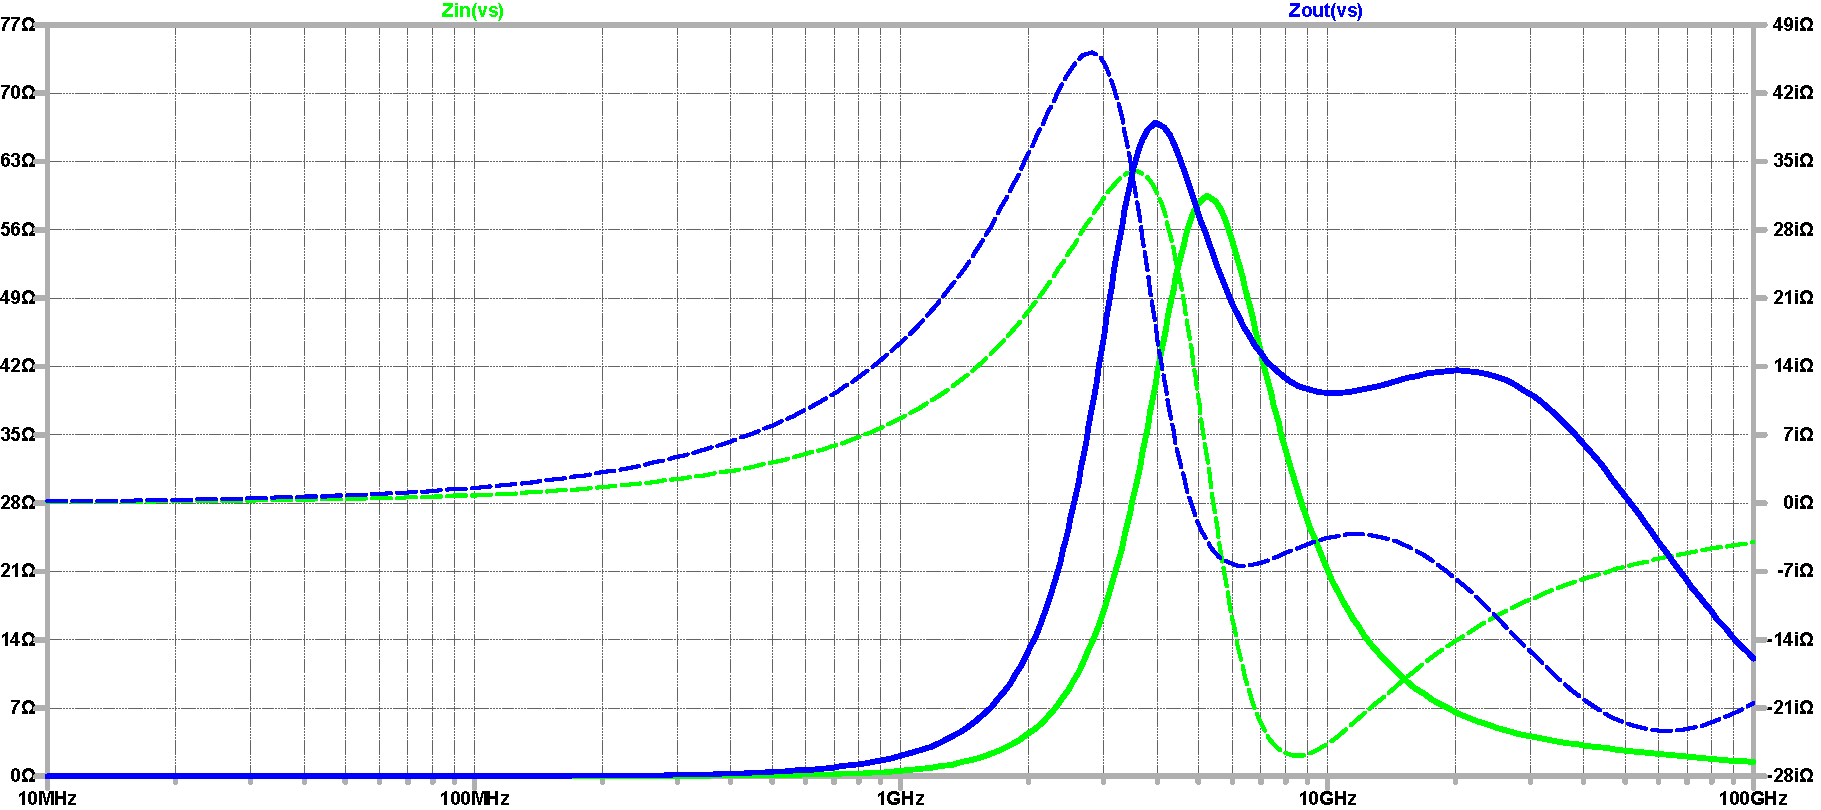
\includegraphics[width=.9\linewidth]{img/q6/zin-zout-s-matched.pdf}
\caption{\label{fig:zin-zout-s-matched-q6}Input and output impedance with minimum S\textsubscript{11} and S\textsubscript{22}.}
\end{figure}

\begin{figure}[H]
\centering
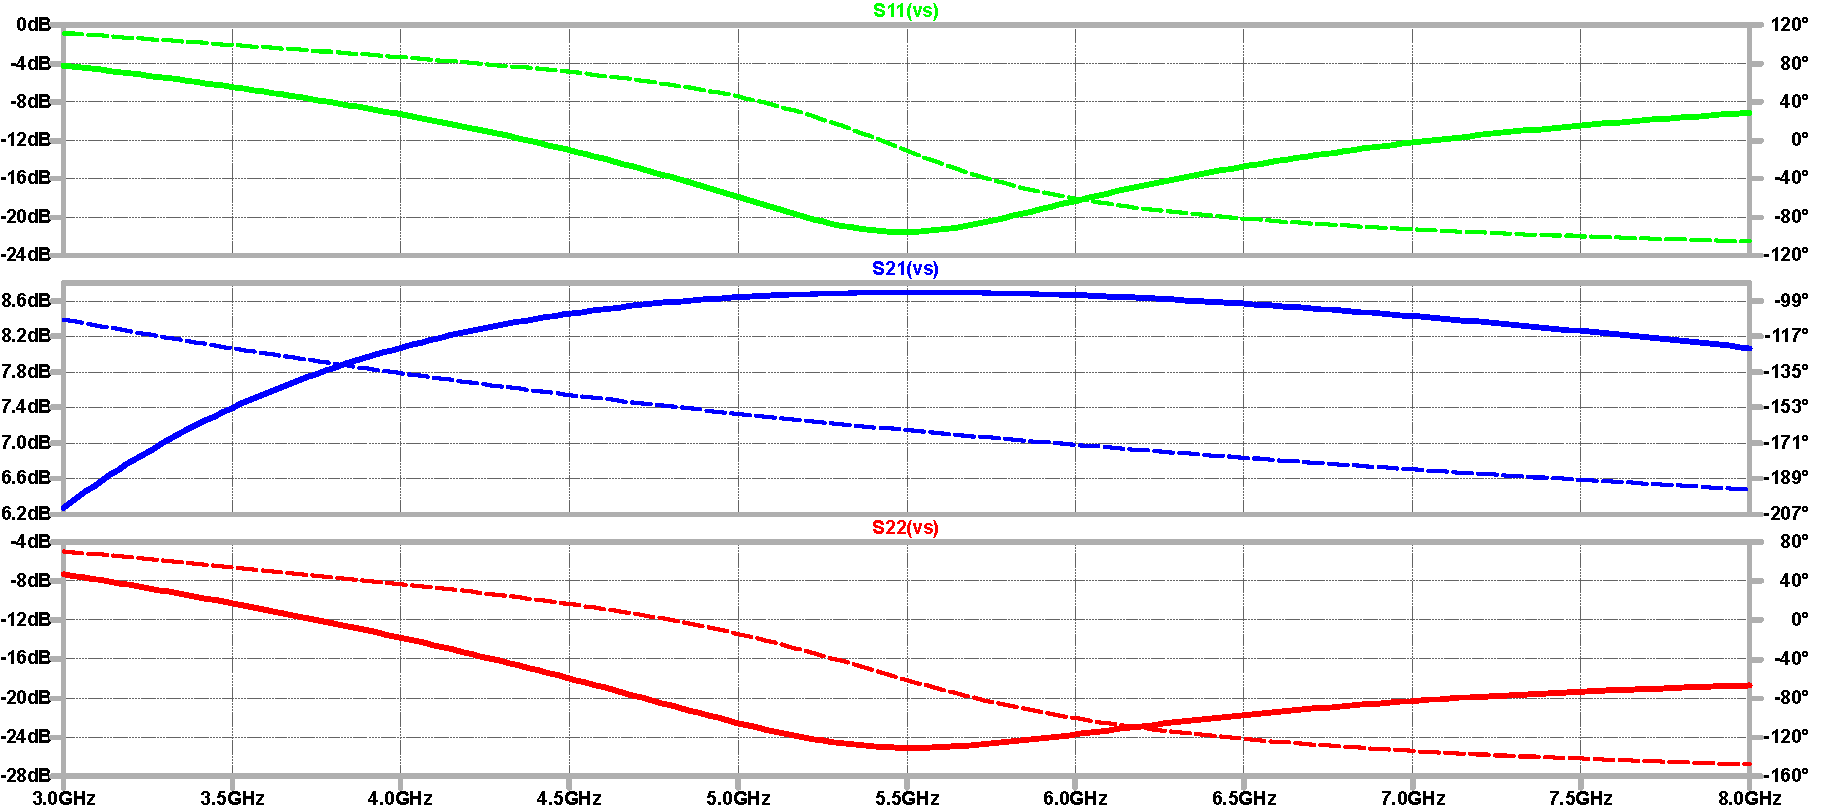
\includegraphics[width=.9\linewidth]{img/q6/s-s-matched.pdf}
\caption{\label{fig:s-param-s-matched-q6}S-parameters with minimum S\textsubscript{11} and S\textsubscript{22}.}
\end{figure}

\begin{figure}[H]
\centering
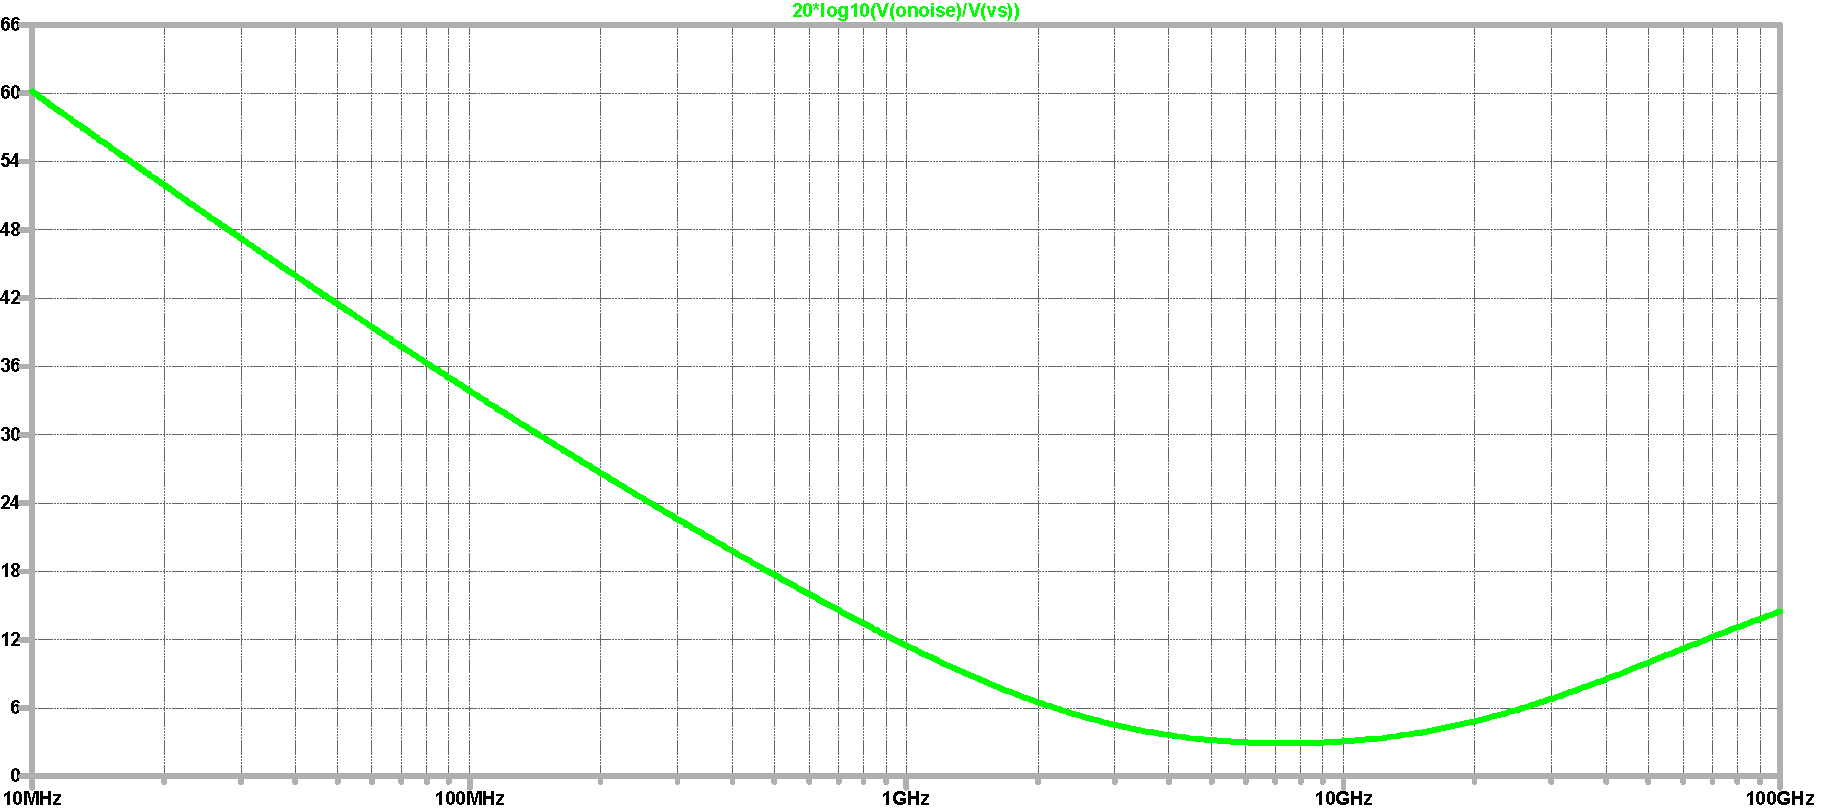
\includegraphics[width=.9\linewidth]{img/q6/noise-s-matched.pdf}
\caption{\label{fig:noise-s-matched-q6}Noise figure with minimum S\textsubscript{11} and S\textsubscript{22}.}
\end{figure}
\end{enumerate}

\item The final design of the LNA have met the required specifications. However, the input and output
impedance matching are not exactly \(50 \Omega\). This can be improved using a cascode stage to
isolate the input and output impedancences. On inspection, the bandwidth of the LNA is small,
further improvements using ``phantom zeroes'' is most likely required.
\end{enumerate}
\end{document}
